\newcommand{\DeinName}{Silvere Sacker Ngoufack}
\newcommand{\TitelArbeit}{LoRa based IoT endpoint and gateway}

\newcommand{\PrueferEins}{Prof. Dr.-Ing. Hartmut Weber}
\newcommand{\PrueferZwei}{Prof. Dr.-Ing. Martin Gr�fe}
\newcommand{\fachbereich}{Informationstechnik - Elektrotechnik - Mechatronik}
% entweder ein Datum h�ndisch eintragen, oder den Befehl \today nutzen
\newcommand{\Datum}{29 April 2020}

\makeglossary


%
% Einbinden des Headers, hier k�nnen auch weitere Einstellungen vorgenommen werden.
%%%%%%%%%%%%%%%%%%%%%%%%%%%%%%%%%%%%%%%%%%%%%%%%%%%%%%%
%																					%
%	In dieser Datei werden alle Packages eingebunden, 	%
% welche f�r das Dokument n�tig sind. Desweiteren 		%
% werden die Dokumentinformationen gesetzt.						%
%																											%
%%%%%%%%%%%%%%%%%%%%%%%%%%%%%%%%%%%%%%%%%%%%%%%%%%%%%%%
%
%	Die KOMAScript Dokumentklasse "scrbook" verwenden.
%
\documentclass[pdftex, 		%
							a4paper, 		% DIN A4 verwenden
							titlepage,	% separate Titelseite
							%draft,			%	Draft-Version, keine Bilder im pdf!
							final,			% Final-Version
							oneside,		% einseitiger Druck
							11pt,				% Schriftgr��e 12pt
							DIV=calc,
							%tocbasic,
							]{scrbook}	%	KOMAScript scrbook-Dokumentklasse
							
%%%%%%%%%%%%%%%%%%%%%%%%%%%%%%%%%%%%%%%%%%%%%%%%%%%%%%%%
%	Einbinden der Pakete 
%%%%%%%%%%%%%%%%%%%%%%%%%%%%%%%%%%%%%%%%%%%%%%%%%%%%%%%%

\usepackage[ngerman]{babel}
%\usepackage[a4paper, top=3.5cm]{geometry}
% PDF Dateien einbinden Das will ich nicht
\usepackage{pdfpages}
\usepackage{endnotes}

%Settings for PDF Pages to accept additonal versioned PDF files
\pdfminorversion=6
\pdfcompresslevel=9
\pdfobjcompresslevel=9


%Einige Pakete haben Probleme mit dem Komaskript.
\usepackage{scrhack} 

% Add url to bibliography
\usepackage{url}


% Definieren von eigenen benannten Farben.
% F�r sp�tere Verwendung in dem Dokument, definieren wir einzelne
% benannte Farben.
%
\usepackage{xcolor}
\definecolor{gray1}{gray}{0.92}
\definecolor{darkgreen}{rgb}{0,0.5,0}

\definecolor{urlLinkColor}{rgb}{0,0,0.5}
\definecolor{LinkColor}{rgb}{0,0,0}
\definecolor{ListingBackground}{rgb}{0.85,0.85,0.85}




\rmfamily
\usepackage{wrapfig} 
\usepackage{natbib}
\usepackage{palatino} 				% Schriftfamilie Palatino
\usepackage[latin1]{inputenc} % Umlaute  
\usepackage{makeidx}   				% Paket zur Erzeugung eines Index
\usepackage[normalem]{ulem}   % bietet Unterstreichungsvarianten
%\usepackage{picins} 					% Bilder im Absatz platzieren
\usepackage[T1]{fontenc}			% Erweiterten Zeichensatz aktivieren
\usepackage[printonlyused]{acronym}
\usepackage{multido}					% erm�glicht Schleifenartiges wiederholen von Befehlen
\usepackage{mdwlist}					% erm�glicht das Setzen des Z�hlers bei Aufz�hlungspunkten
\usepackage{paralist}					% Paket f�r Aufz�hlungen, erweitert Enumerate-Paket
\usepackage{longtable}				% mehrseitige Tabellen
\usepackage{tocbasic}
\parindent0pt           			% verzichte auf Einr�cken der ersten Zeile
\parskip1ex             			% Abstand zwischen den Abs�tzen

\usepackage{setspace}					% Paket zum Einstellen des Zeilenabstands
\onehalfspacing								% anderthalbfacher Zeilenabstand
%\doublespacing								% doppelter Zeilenabstand
%\singlespacing								% einfacher Zeilenabstand

%\usepackage[german]{babel}
\usepackage[german=quotes]{csquotes} %Deutsche Anf�hrungszeichen

\usepackage{color}
\definecolor{LinkColor}{rgb}{0.1,0.1,0.1}
%\definecolor{ListingBackground}{rgb}{0.85,0.85,0.85}
\definecolor{ListingBackground}{rgb}{0.98,0.98,0.98}
\definecolor{gray}{rgb}{0.4,0.4,0.4}
\definecolor{darkblue}{rgb}{0.0,0.0,0.6}
\definecolor{cyan}{rgb}{0.0,0.6,0.6}


%
% Farbeinstellungen f�r die Links im PDF Dokument.
%
\makeindex

%-----------Paket f�r absolute Positionierung von Grafiken------------------
\usepackage[absolute]{textpos}
\setlength{\TPHorizModule}{1mm}
\setlength{\TPVertModule}{\TPHorizModule}

%-----------Aufz�hlungen und Einstellungen f�r Sourcecode-------------------
%\usepackage[savemem]{listings} %Bei wenig Arbeitsspeicher dies Option [savemem] aktivieren.
\usepackage{listings}
\lstloadlanguages{TeX,XML, C} % TeX sprache laden, notwendig wegen option 'savemem'
\lstset{%
	language=[LaTeX]TeX,     % Sprache des Quellcodes ist TeX
	numbers=left,            % Zelennummern links
	stepnumber=1,            % Jede Zeile nummerieren.
	numbersep=5pt,           % 5pt Abstand zum Quellcode
	numberstyle=\tiny,       % Zeichengr�sse 'tiny' f�r die Nummern.
	breaklines=true,         % Zeilen umbrechen wenn notwendig.
	breakautoindent=true,    % Nach dem Zeilenumbruch Zeile einr�cken.
	postbreak=\space,        % Bei Leerzeichen umbrechen.
	tabsize=2,               % Tabulatorgr�sse 2
	basicstyle=\ttfamily\footnotesize, % Nichtproportionale Schrift, klein f�r den Quellcode
	showspaces=false,        % Leerzeichen nicht anzeigen.
	showstringspaces=false,  % Leerzeichen auch in Strings ('') nicht anzeigen.
	extendedchars=true,      % Alle Zeichen vom Latin1 Zeichensatz anzeigen.
	backgroundcolor=\color{ListingBackground}} % Hintergrundfarbe des Quellcodes setzen.


\lstset{
  basicstyle=\small\ttfamily,
  columns=fullflexible,
  showstringspaces=false,
  %commentstyle=\color{gray}\upshape
}
%neue Lang definieren, als Bsp.
\lstdefinelanguage{XML-changed}
{
  basicstyle=\footnotesize\ttfamily\bfseries,
  morestring=[b]",
  morestring=[s]{>}{<},
  morecomment=[s]{<?}{?>},
  stringstyle=\color{black},
  identifierstyle=\color{darkblue},
  keywordstyle=\color{cyan},
  morekeywords={xmlns,version,type}% list your attributes here
}

%-----------Caption Package-------------------
\usepackage{caption}
\DeclareCaptionFont{white}{\color{white}}
\DeclareCaptionFormat{listing}{\colorbox[cmyk]{0.43, 0.35, 0.35,0.01}{\parbox{\textwidth}{\hspace{15pt}#1#2#3}}}

\DeclareCaptionFormat{graphics}{\colorbox[cmyk]{0.43, 0.35, 0.35,0.01}{\parbox{\textwidth}{\hspace{15pt}#1#2#3}}}


\captionsetup[lstlisting]{format=listing,labelfont=white,textfont=white, singlelinecheck=false, margin=0pt, font={footnotesize}}

%-----------Header+Footer---------------------------------------------------
\usepackage{fancyhdr}					%
\pagestyle{fancy}							%
%\rhead[\leftmark]{\thepage}
%\lhead[\thepage]{\rightmark}
\fancyhead{}
\fancyfoot{} 
\renewcommand{\headrulewidth}{0.4pt} % Kopzeilenlinie
\renewcommand{\footrulewidth}{0.0pt} % Fusszeilenlinie 0.0pt blendet sie aus

\renewcommand{\chaptermark}[1]{\markboth{\thechapter\quad#1}{}}
\renewcommand{\sectionmark}[1]{\markright{\thesection\quad#1}}

\fancyhead[LO]{\small\sffamily\rightmark}
\fancyhead[RO]{\small\sffamily\thepage}

% Fu�zeile bearbeiten
\usepackage{geometry}
\geometry{
	bottom=3cm,
	footskip=1cm
}

%-----------Um die Eidesstattliche Erkl�rung als PDF einzubinden-----------------------------------
%\usepackage{pdfpages}

%------------Glossar--------------------------------------------------------------
\usepackage{expdlist}
\usepackage{glossar}

\renewcommand{\glshead}{\chapter*{Glossar}}
\renewcommand{\glentry}[2]{\glossary{#1@[#1] #2|glspage}}
\renewcommand{\glsgroup}[1]{{\listpart{\makebox[0pt][l]{\rule[-2pt]{\textwidth}{0.5pt}}{\textbf{\large #1}}}}}

\makeglossary


% -------F�r ToDo-Notes--------------------------------------------------------------------
\usepackage[color=red, shadow]{todonotes} % ", disable" deaktiviert ToDo-Notes
%Vereinfachtes "Inline-Todo"
\newcommand{\td}[1]{{\todo[inline]{#1}}}
\newcommand{\tdu}[1]{{\todo[inline, color=green!40]{#1}}}

%--------F�r Links-------------------------------------------------------------------------




%--------HyperRef konfigurieren-------------------------------------------------------------------------

\usepackage[
	pdftitle={\TitelArbeit},
	pdfauthor={\DeinName},
	pdfsubject={\TitelArbeit},
	pdfcreator={MiKTeX, LaTeX with hyperref and KOMA-Script auf Basis der Vorlage von seiler.it},
	pdfkeywords={Abschlussarbeit, Mittelhessen, Technische Hoschule},%weitere Keywords hier einf�gen
	pdfpagemode=UseOutlines,%                                  
	pdfdisplaydoctitle=true,%                                  
	pdflang=de%                                              
]{hyperref}

\hypersetup{%
	colorlinks=true,%        Aktivieren von farbigen Links im Dokument (keine Rahmen)
	linkcolor=LinkColor,%    Farbe festlegen.
	citecolor=LinkColor,%    Farbe festlegen.
	filecolor=LinkColor,%    Farbe festlegen.
	menucolor=LinkColor,%    Farbe festlegen.
	urlcolor=LinkColor,%     Farbe von URL's im Dokument.
	bookmarksnumbered=true%  �berschriftsnummerierung im PDF Inhalt anzeigen.
}



% Beginn des Dokuments
\begin{document}


%Zitiert alle Referenzen, ohne Sie hier zu listen. Dadurch erscheinen alle Quellen im %Literaturverzeichnis, auch wenn sie im Text nicht genutzt werden.
%Bitte nur f�r Testzwecke verwenden.
\nocite{*}


% Einbinden des Deckblatts

\frontmatter
% erste Seite (Titelseite) der Bachelorarbeit mit Titel, Name usw...

\newsavebox{\Prof}
\savebox{\Prof}{Erster Pr�fer: }

\newsavebox{\Betr}
\savebox{\Betr}{Zweiter Pr�fer: }



\begin{titlepage}

\begin{textblock}{0}(20,10)
	
\includegraphics[height=2cm]{source/images/THMlogo.png}	
\end{textblock}

\begin{textblock}{20}(165,10)
	
\includegraphics[height=2cm]{source/images/logo-print-hd.jpg}
\end{textblock}

\begin{center}
%\includegraphics[height=2cm]{source/images/logo_mirolab.png}

{\large Technische Hochschule Mittelhessen}\\[1mm]
{\small Fachbereich \fachbereich}
\vspace{1.5cm}

{\huge \TitelArbeit}

\vspace{2cm}

{\large Bachelorarbeit}

\vspace{1.5cm}

von\\[2mm]

\textbf{\large{\DeinName}}\\
\vspace{1.5cm}

Betreuer: John Madieu\\[2mm]

\usebox{\Prof \PrueferEins} \\
\usebox{\Betr \PrueferZwei} \\

\vspace{1.5cm}
Friedberg, den \today
\end{center}

\end{titlepage}

\setcounter{page}{1} %Seitennummerierung ab Seite 2


\chapter{ Abstract} \label{Abstract}	
\enquote{Die Ziele des IoT sind die IT-Vernetzung von Gegenst"anden und 
die Bereitstellung von funktionalit"aten Beziehungsweise 
Dienstleistungen, wie es so noch nie gab.} Das Internet der Dinge ist 
eine zentrale Bedeutung f"ur das Privatleben und die Wirtschaft geworden, 
da ein riesiger Anteil an vernetzten Objekten miteinander kommunizieren. 
Es entstehen neu Einsatzgebiete und Anwendungen mit dem Einsatz 
hochmoderner Technologien. 

Durch den sofortigen Zugriff auf Informationen "uber die Umwelt und die 
Objekte erh"ohen sich Effizienz und Produktivit"at, wodurch sich gro\ss{}e 
Chancen f"ur due Wirtschaft und das Privatleben er"offnen. Der Einsatz des 
IoT erm"oglicht es, umfangreiche Echtzeitinformationen aus der Umwelt 
oder  vom beweglichen und bewegungslose Objekte zu ber"ucksichtigen. Die 
Vorteile sind unter anderen, die zeitliche Verfolgung von Gegenst"ande.

Diese Arbeit besch"aftig sich mit der Entwicklung eines IoT-Endger"at, das 
auf der LoRa-Technilogie und einem STM32L4-Mikrocontroller basiert ist. 
Diese IoT-Endger"at erfasst und sammelt sowohl Umwelt-Daten, wie
Temperatur und Feuchtigkeit, als auch die Beschleunigung. Diese Daten 
werden "uber das LoRa-WAN-Protokol an einem Embedded-Linux basiertes 
Gateway gesendet, entweder lokal in diesem Gateway verarbeitet oder 
diesmal "uber das Internet an einem Anwendungsserver weitergeleitet. 


\newpage





\chapter{Danksagung}
Ich m"ochte mich an dieser Stelle bei allen derjenigen bedanken, die mich w"ahrend der Anfertigung dieser Bachelorarbeit unterst"utzt und motiviert haben.

Zuerst bedanke ich mich herzlich bei John Martial Madieu mein Chef. F"ur seine hilfreichen Anregungen und seine konstruktiven Kritiken sowie seine interessanten Tipps bei der Entwicklung dieser Arbeit m"ochte ich mich bedanken.

Herrn Prof. Dr. Ing. Hartmut Weber und Herrn Prof. Dr. Ing. Martin Gr"afe danke ich f"ur die "Ubernahme und die Betreuung sowohl f"ur diese Arbeit als auch f"ur mein Bachelorstudium.

Ich bedanke mich bei meiner Eltern, Rapha"el und Elvire Kenfack, daf"ur das sie mich immer unterst"utzt haben, und meine bisherige Ausbildung, welches nach dieser Arbeit zum Master weitergeht, erm"oglicht haben. 

Ein besonderer Dank gilt meiner Freundin und meinen Freunden, die durch ihre Fragen und Anmerkungen mein Wissen erweitert haben.\\
\\[6ex]
 
%
% EOF
%

\chapter{Eidesstattliche Erkl�rung}
Hiermit versichere ich, \DeinName, die vorliegende Arbeit selbstst�ndig und ausschlie�lich unter Verwendung
der angegebenen Quellen und Hilfsmittel verfasst zu haben. Inhalte dieser Arbeit, die w�rtlich
oder sinngem�� aus den Quellen entnommen wurden, sind als solche kenntlich gemacht.
Die Arbeit oder Teile daraus wurden in dieser oder vergleichbarer Form noch keinem anderem Pr�fungsgremium vorgelegt und auch nicht ver�ffentlicht.\\
\\[6ex]

Fiedberg, den 03. August 2020


\rule[-0.2cm]{5cm}{0.5pt}

\textsc{\DeinName} 



\tableofcontents 

\backmatter
%Einbinden des Tabellenverzeichnisses
\listoffigures
%Liste der Tabellen
\listoftables
\chapter{Abk"urzungsverzeichnis}

\begin{acronym}[slmtA]
	\acro{IoT}{Internet of Things}
	\acro{LoRa}{Long Range}
	\acro{GSM}{Global System for Mobile Communications}
	\acro{GPS}{Global Positioning System}
	\acro{Kbps}{kilobit per second}
	\acro{UART}{Universal Asynchronous Receiver Transmitter}
	\acro{I2C}{Inter-Integrated Circuit}
	\acro{RF}{Radio Frequency}
	\acro{SPI}{Serial Peripheral Interface}	
	\acro{BLE}{Bluetooth Low Energie}
	\acro{ADC}{Analog Digital Converter}
	\acro{LSB}{Less Significant Bit}
	\acro{RH}{Relative Humidity}
	\acro{MCU}{Microcontroller uni}
	\acro{dps}{Degrees per second}
	\acro{SMD}{Surface-Mounted Device}
	\acro{ODR}{Output Data Rate}
	\acro{LPUART}{Low Power UART}
	\acro{FSK}{Frequency Shifting Keying}
	\acro{SF}{Speading Factor}
	\acro{NwkSKey}{Network Session Key}
	\acro{AppSKey}{application Session Key}
	\acro{DevEUI}{Device Unique Identifier}
	\acro{MIC}{Message Integrity Code }
	\acro{MAC}{media access control address}
	\acro{OTAA}{Over-The-Air Activation}
	\acro{ABP}{Activation By Personalization}
	\acro{ADR}{Adaptive Data Rate}
	\acro{dBm}{(Decibel miliwatt}
	\acro{MQTT}{Message Queuing Telemetry Transport}
	\acro{HTTP}{Hypertext Transfer Protocol}
	\acro{TCP}{Transmission Control Protocol}
	\acro{CSV}{Comma-Separated Values}
\end{acronym}

%Einbinden des Hauptteils
\mainmatter

\chapter{Einleitung}

Dieses Kapitel soll den Leser auf den Inhalt der Arbeit aufmerksam 
machen, ihn mit der Aufgabestellung vertraut machen und "uber die 
Strukturierung und Zielsetzung der Arbeit Auskunft geben.


\section{Motivation}
Objekte werden in der heutigen Tagen immer mehr mit Elektronik und 
Intelligenz versehen. Die Leute wollen aufgrund dieser Entwicklung, dass 
Prozesse oder bestimmte Aufgaben ohne menschliches Eingreifen erledigt 
und miteinander vernetzt werden. Das System soll nur "uberwacht werden 
und die Ergebnisse zu bestimmten Zwecken benutzt werden.

Das Internet der Dinge (in Englisch \textbf{\textit{internet of 
things}}, Kurzform \textbf{IoT}) wird dazu benutzt, um die 
Interaktionzwischen Menschen und vernetzten elektronischen Ger"aten zu 
vereinfachen. 


\section{Aufgabenstellung und Zielsetzung}
Man m"ochte Daten wie Energieverbrauch eines Hauses, Bewegung eines 
Objekts oder die Temperatur eines Raums kennen und "uber lange Strecken 
(20Km) "ubertagen ohne hohe kosten mit aber hohe Batterielaufzeit. Es 
gibt heutzutage Technologien wir GSM, Bluetooth oder Wifi, die diese 
Arbeit erledigen k"onnen. Das Problem dabei ist, dass es beim Nutzen von 
GSM hohe Lizenzkosten fallen mussen. Was Bluetooth und Wifi betrifft, 
sind ihre Reichweite sehr kurz. Dieser Ziel kann mit Hilfe der 
LoRa-Technologie erreicht werden, da sie diese Nachteilen beseitigt.  

In dieser Abschlussarbeit soll ein Prototyp gebaut werden, der mit Hilfe
der LoRa-Technologie Daten an einem Server senden und von diesem Server 
Daten Empfangen. Anders gesagt, diese Bachelorarbeit besch"aftigt sich 
mit der Entwicklung eines vernetzten Systems bestehend aus einem 
3D-Beschleunigungssensor, einem 3D-Gyroskop sowie einem Tem\-peratur- 
und Feuchtigkeitssensor. Die Sensoren messen Daten und "ubergeben diese 
an den STM32L475 Mikrocontroller.

Der Mikrocontroller soll die Daten verarbeiten und mit Hilfe eines 
LoRa-Moduls\cite{AT_Command} drahtlos an einem Server "ubertragen. Bevor 
die "Ubertragung erfolgt, muss das LoRa-Endger"at Zugang zu dem Neztwerk 
durch dem Server bekommen. Nach dem das LoRa-Endger"at dem Netzwerk 
hinzugef"ugt wurde, k"onnen nun Informationen zwischen dem 
LoRa-Endger"at und dem Netzwerk-Server bis zu einem Anwendungsserver 
vertauscht werden. Abbildungen \ref{fig:LRWAN} und 
\ref{fig:LabcsmartLoRawan} geben einen "Uberblick "uber den Aufbau des 
gesamten Systems.

\vspace{2cm}
\begin{figure}[h]
	\centering
	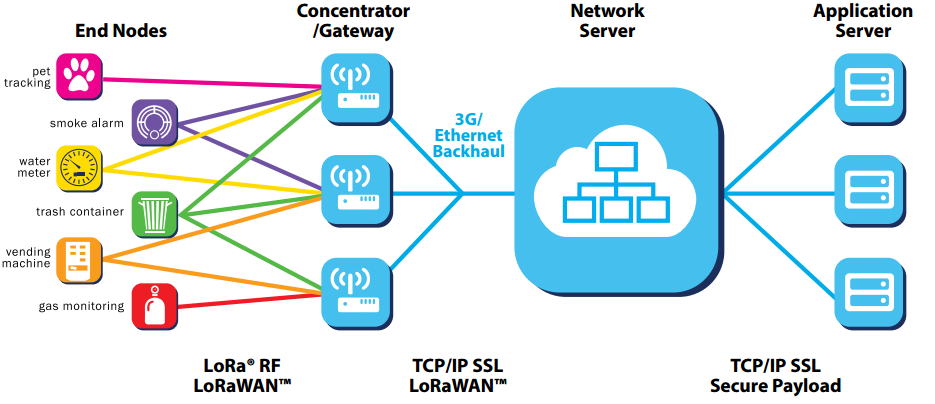
\includegraphics[width=15cm]{source/images/LoRaWAN_NET}
	\caption{Allgemeine LoRaWAN Netzwerkarchitektur 
	\cite{LoRaWAN}\label{fig:LRWAN}}
\end{figure}


\begin{figure}[h]
	\centering
	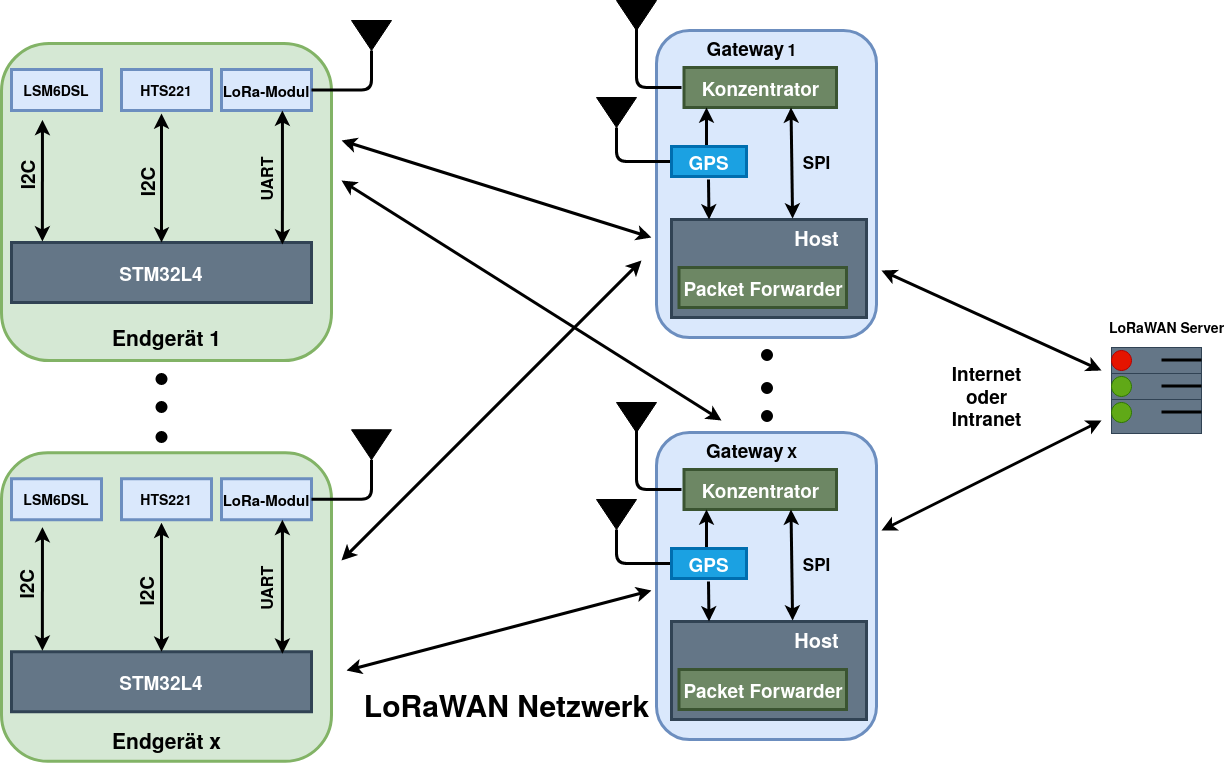
\includegraphics[width=15cm]{source/images/Gesamtsystem}
	\caption{Labcsmart LoRaWAN Netzwerk \label{fig:LabcsmartLoRawan}}
\end{figure}

\begin{description}
	\newpage
	\item[LoRa:] ist eine abk"urzung f"ur \textbf{\textit{Long Range}} 
	und es ist eine drahtlose Technologie, das geringe Sendeleistung 
	verbraucht wird, um kleine Datenpakete (0,3 Kbps bis 5,5 Kbps) "uber 
	eine lange Strecke zu senden oder zu empfangen.    
	
	\item[End Node Endger"at:] ist ein Ger"at, das aus zwei Teilen 
	Besteht. Ein Funkmodul mit Antenne und einem Mikrocontroller zur 
	Verarbeitung der Daten wie Sensordaten. Diese Daten k"onnen entweder 
	an einem anderen LoRa-Node per Point-To-Point-Verbindung oder an 
	einem LoRaWAN-Netzwerk versand werden.

	\item[LoRaWAN:] steht f"ur \textbf{\textit{Long Range Wide Area 
	Network}} und ist das Kommunicationsprotokol f"ur den Netzwerk.
	
	\item[Gateway:] ist ein Ger"at, das aus mindestens einem 
	Funkkonzentrator, einem Host und einer Netzverbindung zum Internet 
	oder einen privaten Netzwerk (Ethernet, 3G, Wifi), m"oglicherweise 
	einem GPS-Empf"anger besteht.
	
	\item[LoRaWAN Server:] ist ein abstrakter Computer, der die von dem 
	Gateway empfangene RF-Pakete verarbeitet und sendet RF-Pakete als 
	Antwort, dass das Gateway zur"ucksenden muss.
	\vspace{1cm}
	\item[Application Server:] ist eine Anwendung, womit der Benutzer 
	die von den Sensoren gemesennen Daten entweder Tabelarisch oder 
	Grafisch ansehen kann.
	
	\item[Uplink:] ist die Kommunikation von einem Endger"at zu einem 
	Gateway. 
	
	\item[Downlink:] ist die Kommunikations von einem Gateway zu einem 
	Endger"at.
\end{description}


\section{Gliederung der Arbeit}

Das Kapitel \ref{Komponente} gibt einen detaillierten "Uberblick "uber 
allen Hardware-Komponenten, die bei der Entwicklung eines Endger"at 
verwendet werden. Als Erstes wird auf die Eigenschaften von des 
benutzten STM32-Nucleo Board eingegangen. Diesem Kapitel ist auch zu 
entnehmen, warum genau dieses Board gew"ahlt wurde. 

Als n"achstes wird das LoRa-Modul. Dieses LoRa-Modul wird dazu 
verwendet, um die gesammelten Daten dem Server drahtlos zu "ubertragen. 
Dieser Kapitel berichtet "uber das Funkprotokol, das zur "Ubertragung 
der Daten eingesetzt wurde, und wie diese Daten gerichert werden.
 
Das Kapitel \ref{G_S} beschreibt den LoRaWAN-Server und das Gateway, 
zwei wichtige Teile dieser Thesis. Die Funktionsweise wird erkl"art und  
die Servereinstellung wird gezeigt. Diese Einstellung sind notwendig, 
weil sie erlauben einem Endger"at denḿ Netzwerk einzutreten.

Als n"achstes wird die Softwareentwicklung behandelt. Hier geht es 
erstmal um die Entwicklungsumgebung des gesamten Projekts (Eclipse). 
Anschlie\ss{}end daran werden die angewante Bibliotheken dargestellt, 
ihre Installation und Nutzung erkl"art. Es wurde f"ur diese Arbeit zwei 
bekannte Kommunikationsschnittstellen verwendet (I2C und UART) Sie 
erfahren auch wie diese Schnittstellen mit der Programmiersprache C 
angesteuert werden, und welche Software-Tricks eingesetzt wurden, um 
AT-Befehle zu senden.

Anschlie\ss{}end  wird im Kapitel \ref{Fazit} eine Zusammenfassung und 
einen kleinen Ausblick der Arbeit gegeben.
   
\chapter{Hardware Komponenten eines Endger"ats}\label{Komponente}

In diesem Kapitel werden die f"ur das Gesamtsystem benutzten 
Hardware- Komponenten hinsichtlich ihrer Funktionsweise und Ansteuerung 
in Einzelnen erl"autert. 

\section{STM32L4 Discovery Kit}\label{LoRa}

Das STM32L4 Discovery Kit ist ein IoT Knoten, womit ein Benutzer 
Anwendungen mit direkter Verbindung zu einem oder mehreren 
Cloud-Servern entwickeln kann.
Dieses Discovery Kit erm\"oglicht eine Vielzahl von Anwendungen, indem 
es eine Multikink-Kommunikation (\ac{BLE}) mit geringem 
Stromverbrauch  Multiway-Erkennung der Umwelt erm"oglicht (Siehe 
Abbildung \ref{Node}).

Das STM32L4 hat einen eingebetteten ST-LINK Debugger/Programmierer, 
eingebettete Sensoren und viele andere Features, die in dem Datenblatt 
\cite{B-L475E-IOT01A} erl"autert zu finden sind. Genau wegen der 
Vielfalt an Eingenschaften wurde dieses Board ausgew"ahlt. Man braucht 
kein Breadboard im Vergleich zu dem Arduino oder dem Raspberry-Pi, um 
die Sensoren mit den Schnittstellen (UART, \ac{SPI} oder I2C) des 
Mikrocontrollers zu verbinden. Noch dazu eignet sich dieses Discovery 
Kit f"ur ein Endger"at von STMicroelectronics, da Arduino-Verbinder 
vorhanden sind. Dazu ist nur das Endger"at in dieser Verbinder stecken. 

\begin{figure}[h]
	\centering
	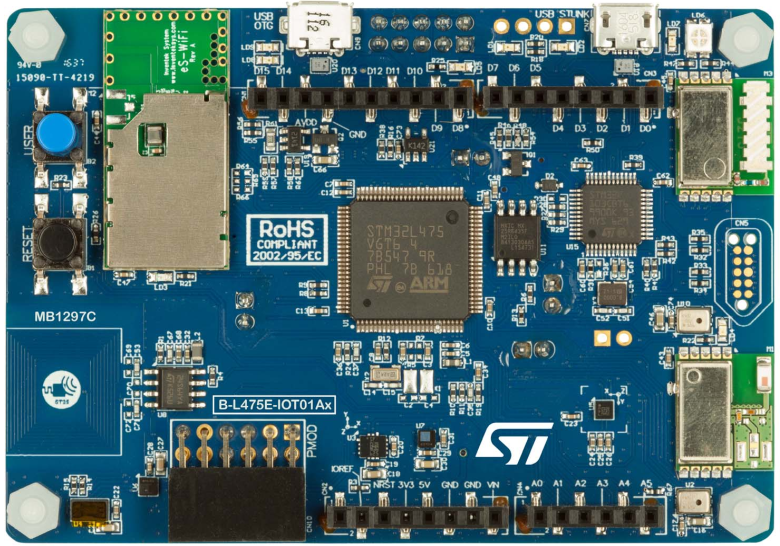
\includegraphics[width=12cm]{source/images/Board}
	\caption{B-L475E-IOT01A Discovery kit 
	\cite{B-L475E-IOT01A}}\label{Node}
\end{figure}

F"ur diese Arbeit werden wir uns auf zwei Sensoren beschr"anken. 
Erstmal den HTS221\cite{HTS221} Temperatur- und Feuchtigkeitssensor 
und dann den LSM6DSK 3D-Gyroscope und 3D-Beschleunigungssensor 
\cite{LSM6DSL}. Diese Daten werden erfasst und drahtlos an den 
LoRaWAN-Server "ubertragen. Die folgenden Unterkapitel beschreiben, 
wie diese Sensoren funktionieren und erkl"aren, wie sie anzusteuern 
sind, damit die erhaltenen Daten im Rahmen der geforderten Toleranzen 
der Realit"at entsprechen. Laut dem Datenblatt ist mit einer 
Temperaturgenauigkeit von \textpm 0.5\textdegree{}c und einer 
Feuchtigkeitsgenauigkeit von \textpm 3.5\%   zu rechnen. 

\subsection {HTS221 Temperatursensor- und Feuchtigkeitssensor}\label{Temp}
In diesem Unterkapitel wird der HTS221 Temperatur- und 
Feuchtigkeitssensor beschrieben und erkl"art wie die Temperatur und 
die Feuchtigkeit zu ermitteln sind.

Der HTS221 Sensor misst die relative Feuchtigkeit(H) und die 
Temperatur (T) und speichert die Daten (16-Bits von Datentyp Integer) 
als Zweierkomplement. Diese Daten k"onnen "uber I2C- oder 
SPI-Schnittstelle gelesen werden. Die gespeicherte Daten sind 
Rohdaten, die am Ausgang von dem \ac{ADC} verf"ugbar sind (Siehe 
Abbildung \ref{HT_sensor}). Um die Temperatur in \textdegree{}c und 
die relative Feuchtigkeit in \% zu bekommen, muss man die Daten aus 
den Registern auslesen und mit Hilfe der Formel \ref{HumFormel} und 
\ref{TempFormel} die richtigen Werten herausfinden.

\begin{figure}[h]
	\centering
	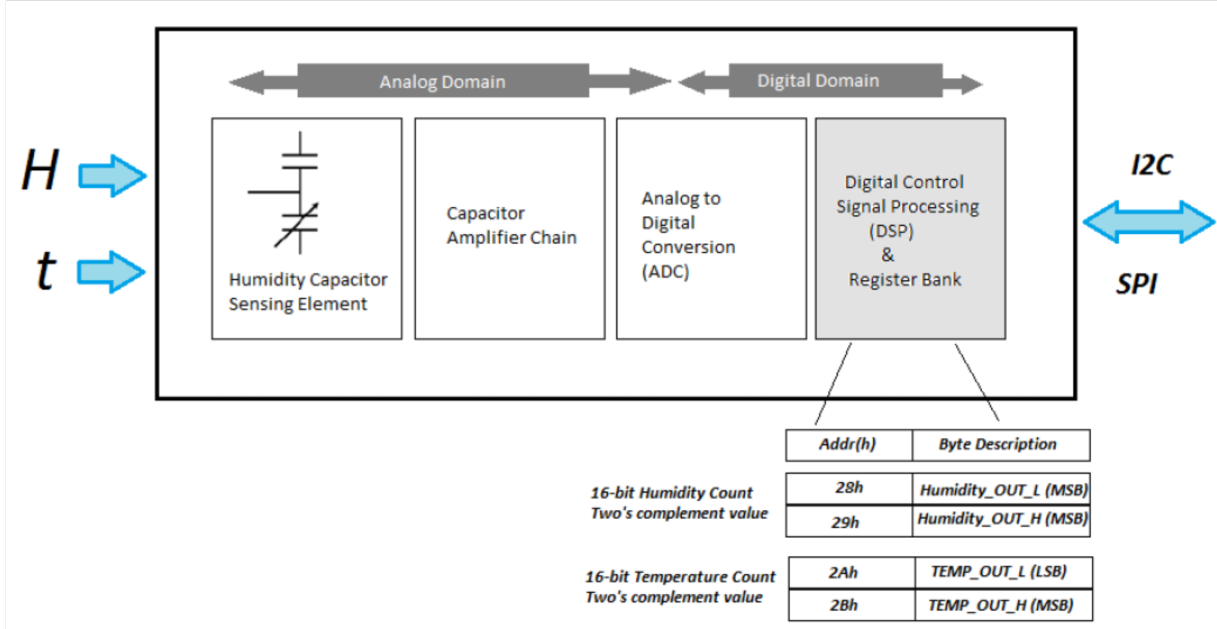
\includegraphics[width=14cm]{source/images/HTS221_sensor}
	\caption{Humidity sensor analog-to-digital flow 
	\cite{HTS221}}\label{HT_sensor}
\end{figure}

\subsubsection{Feuchtigkeit ermitteln}

An dieser Stelle wird erkl"art wie die Feuchtigkeit von dem Sensor 
ermittelt wird.
Der HTS221 Sensor speichert den Feuchtigkeitswert in Rohz"alungen in 
zwei 8-Bit-Registern:
\begin{itemize}
	\item \textit{H\_OUT\_H} (0x29) (H"ochstwertige Bits)
	\item \textit{H\_OUT\_L} (0x28) (Niedrigswertige Bits)
\end{itemize}

Die zwei Bytes werden verkettet, um ein Zweierkomplement dargestelltes 
16-Bit Wort zu bilden. Der relative Feuchtigkeitswert muss durch 
lineare Interpolation
der Register (\textit{HUMIDITY\_OUT\_H} \& \textit{HUMIDITY\_OUT\_L}) 
mit den Kalibrierregistern berechnet werden.

Der HTS221 Sensor ist bei der Herstellung schon kalibriert und die 
erforderlichen Koeffizienten sind ADC 16-Bit-Werte, die in den  
Registern des Sensors zu lesen sind. Eine weitere Kalibrierung durch den 
Benutzer ist nicht erforderlich.

Die Tabelle \ref{tab:Reg_H} stellt die Register dar, in dem die 
Kalibrierwerte zur Ermittlung der relativen Feuchtigkeit gespeichert 
sind.

\vspace{2cm}
\begin{center}
	\begin{table}[htbp] 
		\centering 
		\Large
	%	\footnote{(u16) 16Bit-Wert ohne Vorzeichen, (s16) 16-Bit-wert 
	%mit Vorzeichen}
		\begin{tabular}{l|c|r}
			\textbf{Variable} & 	\textbf{Adresse} & 
			\textbf{Format}\footnotemark\\
			\hline
			\textit{H0\_rH\_x2}	& 0x30	& u(8) \\
			\hline
			\textit{H1\_rH\_x2}	& 0x31	& u(8)\\
			\hline
			\textit{H0\_TO\_OUT\_H} & 0x36	& s(16)\\
			\hline
			\textit{H0\_TO\_OUT\_L} 	& 0x37  & s(16)\\
			\hline
			\textit{H1\_TO\_OUT\_H}	& 0x3A	& s(16)\\
			\hline
			\textit{H1\_TO\_OUT\_L} 	& 0x3B  & s(16)\
		\end{tabular} 
		\caption{Kalibrierregister f"ur relative Feuchtigkeit} 
		\label{tab:Reg_H} 
		 
	\end{table}
\end{center}
\footnotetext{(u8) 16Bit-Wert ohne Vorzeichen, (s16) 16Bit-Wert mit 
Vorzeichen}

Nun wissen wir welche Register zu lesen sind, damit die relative 
Feuchtigkeit mithilfe der Interpolation berechnet wird. Die folgenden 
Schritten m"ussen vor der Berechnung durchgef"uhrt werden:

\begin{itemize}
	\item Werte von \textit{H0\_rH\_x2} und \textit{H1\_rH\_x2} aus 
	Registern 0x30 und 0x31 lesen 
	\item \textit{H0\_rH\_x2} und \textit{H1\_rH\_x2} durch zwei teilen
	\item Werte von \textit{H0\_TO\_OUT} aus Registern 0x36 und 0x37 
	lesen 
	\item Werte von \textit{H1\_TO\_OUT} aus Registern 0x3A und 0x3B 
	lesen
	\item Rohdate von \textit{H\_T\_OUT} aus Registern 0x28 und 0x29 
	lesen
\end{itemize}

Nachdem diese Register gelesen wurden, kann nun die Berechnung der 
relativen Feuchtigkeit erfolgen.

\begin{figure}[h]
	\centering
	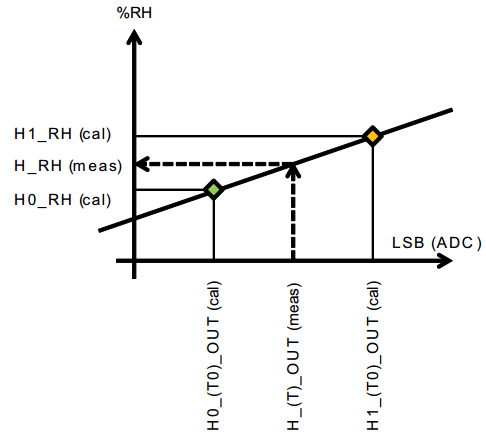
\includegraphics[width=9cm]{source/images/rH}
	\caption{Linear interpolation to convert \ac{LSB} to \%\ac{RH}
	\cite{HTS221}}\label{fig:rH}
\end{figure}

Aus Abbildung \ref{fig:rH} bekommt man mit Interpolation folgende 
Formel \cite{HTS221}:

\begin{center}
	\[
	RH\% = \frac{((H1\_rH - H0\_rH) . (H\_T\_OUT - 
	H0\_T0\_OUT))}{(H1\_T0\_OUT - H1\_T0\_OUT) } + H0\_rH  
	\]\label{HumFormel}
\end{center}

\vspace{10cm}
\subsubsection{Temperatur ermitteln}
Der HTS221 Sensor speichert die Temperaturwerten in Rohz"alungen in 
zwei 8-Bit-Registern:

\begin{itemize}
	\item \textit{T\_OUT\_H} (0x2A) (H"ochstwertige Bits)
	\item \textit{T\_OUT\_L} (0x2B) (Niedrigswertige Bits)
\end{itemize}

Die zwei Bytes werden verkettet, um ein zweierkomplement dargestelltes 
16-Bit Wort zu bilden. Die Polarit"at wird duch den h"ochstwertigen Bit 
vom \textit{T\_OUT\_H} Register bekannt gegeben.

\begin{itemize}
	\item Ist dieser Bit 0, die gelesene Temperatur ist positiv.
	\item Ist dieser Bit 1, die gelesene Temperatur ist negativ. In 
	diesem fall ist das Zweierkomplement des gesamten Wort zu bilden, 
	um den richtigen Wert zu bekommen.
\end{itemize}

Auch hier ist die Temperatur durch lineare Interpolation von den 
Kalibrierregistern und den Registern \textit{T\_OUT\_H} und 
\textit{T\_OUT\_H} in Zweierkomplement zu berechnen.

Die Tabelle \ref{tab:Reg_T} stellt diese Kalibrierregister dar.

\begin{center}
	\begin{table}[htbp] 
		\centering 
		\Large
		%	\footnote{(u16) 16Bit-Wert ohne Vorzeichen, (s16) 
		%16-Bit-wert mit Vorzeichen}
		\begin{tabular}{l|c|r}
			\textbf{Registern} & \textbf{Adresse} & \textbf{Format} \\
			\hline
			\textit{T0\_degC\_x8} & 0x32	& u(8) \\
			\hline
			\textit{T1\_degC\_x8} & 0x33	& u(8)\\
			\hline
			\textit{T1/TOmsb} & 0x35	& (u2),(u2)\\
			\hline
			\textit{T0\_OUT\_H} 	& 0x3D  & s(16)\\
			\hline
			\textit{T0\_OUT\_L} 	& 0x3C  & s(16)\\
			\hline
			\textit{T1\_OUT\_H}	& 0x3F	& s(16)\\
			\hline
			\textit{T1\_OUT\_L} 	& 0x3E  & s(16)\
		\end{tabular} 
		\caption{Kalibrierregister zur Temperaturermitllung} 
		\label{tab:Reg_T} 
		
	\end{table}
\end{center}

Da die Kalibrierregister vom Hersteller mit den korrekten Werten 
versehen werden, werden wir nun diese Register lesen und mithilfe der 
gelesenen Werten die Temperatur ermitteln. Bevor man die Temperatur 
mit linearer Interpolation berechnet, sind folgende Schritten 
erstmal erforderlich.

\begin{itemize}
	\item Die Koeffiziente \textit{T0\_degC\_x8} und 
	\textit{T1\_degC\_x8} aus den Registern 0x32 und 0x33 lesen
	\item Die Werte von \textit{T0\_degC\_x8} und \textit{T1\_degC\_x8} 
	durch 8 divisiren, um die Koeffiziente \textit{T0\_degC} und 
	\textit{T1\_degC} zu bekommen.
	\item Die h"ochstwertige Bits von T\textit{1\_degC}(T1.9 und T1.8) 
	und \textit{T0\_degC}(T0.9 und T0.8) aus dem Register 0x35 lesen. 
	Diese Werte an den im Schritt 2 ermittelten Werten verketten, damit 
	\textit{T0\_degC} und \textit{T1\_degC} vollst"andig werden.
	\item Der Wert von \textit{T0\_OUT} aus den Registern 0x3C und 0x3D 
	lesen.
	\item Der Wert von \textit{T1\_OUT} aus den Registern 0x3E und 0x3F 
	lesen.
	\item Der Wert von \textit{T\_OUT} aus den Registern 0x2A und 0x2B 
	lesen.
	 	
\end{itemize}

Nachdem diese Kallibrierregister gelesen wurden, kann man mittels 
linearer Interpolation die Temperatur in \textdegree{}c berechnen.

\begin{figure}[h]
	\centering
	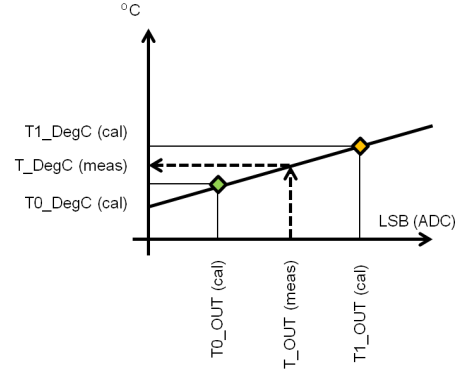
\includegraphics[width=9cm]{source/images/Temp}
	\caption{Linear interpolation to convert LSB to \textdegree{}c 
	\cite{HTS221}}\label{fig:T}
\end{figure}

Abbildung \ref{fig:T} zeigt der Graph woraus die lineare Interpolation 
stammt. Die folgende Formel wurde sogar daraus hergeleitet.

\begin{center}
	\[
	T[\textdegree{}c] = \frac{((T1\_degC - T0\_degC) . (T\_OUT - 
	T0\_OUT))}{(T1\_OUT - T0\_OUT) } + T0\_degC  
	\]\label{TempFormel}
\end{center}

Da die Kalibrierwerten zur Berechnung der Temperatur und der relativen 
Feuchtigkeit bei der Herstellung des Bausteins vorab festgesetzt sind, 
soll man die Kalibrierregister bei der Programmierung nur ein mal 
auslesen. Dies erspart den Rechenaufwand des Mikrocontrollers.
 
\subsection{LSM6DSL 3D Gyroskope und 3D Beschleunigungssensor}\label{Acc/Gy}

Dieses Unterkapitel berichtet von dem LSM6DSL 3D-Gyroskope und 
3D-Besch-leunigungssensor. Hier ist zu entnehmen, wie die X-,Y-, und 
Z-Koordinaten der Sensoren zu ermitteln sind und wie der Sensor 
abh"angig vom Zweck skaliert werden kann.
 

Der LSM6DSL ist ein digitaler 3D-Beschleunigungsmesser und ein 
3D-Gyroskop-system mit einer digitalen seriellen I2C/SPI Schnittstelle 
mit einer leistung von 0.65mA im kombinierten Hochleistungsmodus.
Das Ger"at verf"ugt "uber einen von Benutzer w"ahlbaren dynamischen 
Beschleunigungsbereich von \textpm 2 \textbar \textpm 4 \textbar 
\textpm 8 \textbar \textpm 16g (g is gleich 9,81m/s) und einen 
Winkelgeschwindigkeitsbereich von \textpm 125 \textbar \textpm 250 
\textbar \textpm 500 \textbar \textpm 1000 \textbar \textpm 2000\ac{dps}
 
Das extrem geringe Gr"o\ss{}e und das geringe Gewicht des \ac{SMD}-Packets 
machen den LSM6DSL zu einer idealen Wahl f"ur tragbare Anwendungen wie 
Smartphones, IoT-verbundene Ger"ate und andere Anwendungen, bei der 
reduzierte Paketgr"o\ss{}e und -gewicht erforderlich sind.  

Der LSM6DSL bietet drei m"ogliche Betriebskonfiguration:
\begin{itemize}
	\item nur Beschleunigungsmesser aktiv und Gyroskope inaktiv
	\item nur Gyroskope aktiv und Beschleunigungsmesser inaktiv
	\item beide aktiv mit unabh"angigem \ac{ODR} 
\end{itemize}

Der Beschleunigungsmesser und der Gyroskop k"onnen unabh"angig 
voneinander konfiguriert werden unter anderem: Power-down, Low-Power, 
Normal- und High -performance Modus. Um den Stromverbrauch des Sensors 
zu reduzieren, kann der Gyroskop in einem Ruhestand gesetzt werden.


Sobald das Ger"at mit Strom versorgt wird, werden die 
Kalibrierkoeffizienten vom eingebettetem Flash-Speicher zu den  
Register. Dieser Vorgang dauert ungef"ahr 15 milisekunden. Nach dieser 
Zeit fallen der Beschleunigungsmesser und der Gyroskop im Power-Down 
Modus. Durch der \textit{CTRL1\_XL} bzw. \textit{CTRL2\_G-}Register 
k"onnen die Ger"ate geweckt werben, indem man das Betriebsmodus 
ausw"ahlt.

Wenn die Daten verf"ugbar sind, wird eine Unterbrechung (Interrupt 
demn"achst) ausgel"ost, wenn der entsprechende Byte vom 
Beschleunigungsmesser bzw. vom Gyroskop in dem \textit{INT1\_CTRL-} 
Register geschrieben wurde. Das vorhandensein der Daten kann nun mithilfe des Statusregisters abgefragt werden. Das \textit{XLDA-}Bit wird 
auf 1 gesetzt, wenn am Ausgang des Beschleunigungsmessers ein neuer 
Datensatz verf"ugbar ist. Das \textit{GDS-}Bit wird suf 1 gesetzt, wenn 
am Gyroskopausgang ein neuer Datensatz verf"ugbar ist.

\begin{figure}[h]
	\centering
	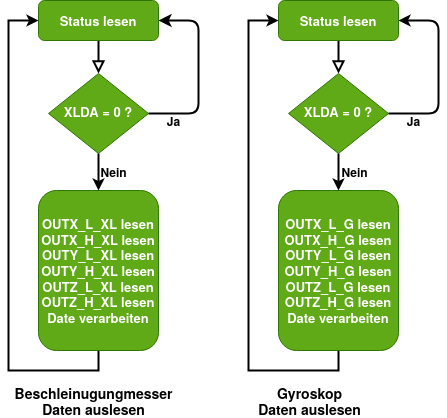
\includegraphics[width=8cm]{source/images/Gy_Acc_data}
	\caption{Flu\ss{}diagram zur Datenermitlung}\label{Gy_Acc_data}
\end{figure}

Das Abbildung \ref{Gy_Acc_data} ist der Flu\ss{}diagram zur Ermittlung 
der Achsen- und Winkelver"anderungen des Beschleunigungsmessers und des 
Gyroskop.

\vspace{10cm}

Wie oben schon erl"autert, kann das Ger"at so eingestellt werden, 
dass ein neuer Satz von Messdaten durch ein Signal erkennbar wird. Das 
\textit{XLDA-}Bit von dem \textit{STATUS\_REG-}Register wird auf 1 
gesetzt, wenn Daten aus dem Beschleunigungsmesser zum Lesen verf"ugbar 
sind. Das Signal kann durch den \textit{INT1-}Pin angesteuert werden, 
indem  das \textit{INT1\_DRDY\_XL-}Bit vom 
\textit{INT1\_CTRL-}Register auf 1 gesetzt wird. 

F"ur den Gyroskopsensor wird das \textit{GDA-}Bit auf 1 gesetzt, wenn 
die Daten zum Lesen verf"ugbar sind. Das Signal kann durch den 
\textit{INT1-}Pin angesteuert werden, indem  das 
\textit{INT1\_DRDY\_G-}Bit vom \textit{INT1\_CTRL-}Register auf 1 
gestezt wird. Die gemessenen Beschleunigungsdaten werden in 
\textit{OUTX\_H\_XL-}, \textit{OUTX\_L\_XL-}, \textit{OU-TY\_H\_XL-}, 
\textit{OUTY\_L\_-XL-}, \textit{OUTZ\_H\_XL-}, 
\textit{OUTZ\_L\_XL-}Register gesendet. Die gemessenen 
Winkelgeschwindigkeitsdaten werden dagegen in \textit{OUTX\_H\_G-}, 
\textit{OUTX\_L\_G-}, \textit{OUTY\_H\_G-}, \textit{OUTY\_L\_G-}, 
\textit{OUTZ\_H\_G-}, \textit{OUTZ\_L\_G-}Register gesendet. Die 
vollst"andigen Ausgangsdaten f"ur die X-,Y- und Z-Achsen sind durch 
die Verkettung von \textit{OUTX\_H\_XL(G)} und 
\textit{OUTX\_L\_-XL(G)},\textit{OUTY\_H\_XL(G)} und 
\textit{OUTY\_L\_XL(G)}, \textit{OUTZ\_H\_XL(G)} und 
\textit{OUTZ\_L\_XL} zu erhalten, wobei die Beschleunigungsdaten und 
die Winkelgeschwindigkeitsdaten als 16-Bit Werte dargestellt sind.

Mit dem LSM6DSL kann man den Inhalt des unteren und oberen Teils der 
Ausgangsdatenregister vertauschen, sodass die Darstellung entweder 
Big-Endian oder Little-Endian entspricht. Dies ist m"oglich, sofern 
man das BLE-Bit von dem CTRL3\_C-Register auf 0 (Little-Endian 
standartm"a\ss{}ig) oder auf 1 (f"ur Big-Endian) Big-Endian bedeutet, 
dass der h"ochstwertige Byte des Datensatzes in der niedrigsten 
Speicherstelle gespeichert wird. Little-Endian bedeutet, dass der 
niedrigswertige Byte des Datensatzes in der niedrigsten Speicherstelle 
gespeichert wird.


Im Unterkapitel \ref{Sensoren} werden die Funktionen zur 
Datenermittlung in der Progra-mmiersprache-C sowohl f"ur den HTS221 
(Temperatur- und Feuchtigkeitssensor) als auch f"ur den LSM6DSL 
(3D-Beschleunigungssensor und 3D-Gyroskop) dargestellt und erkl"art wie 
die Kommunikationsschnittstelle (hier I2C) zu benutzen ist.


\section{LoRa Endger"at: i-nucleo-lrwan1}\label{LoRa Modul}

Die im Kapitel \ref{Temp} ermittelten Sensordaten sollen laut der 
Aufgabestellung mit Hilfe eines drahtloses Protokoll an einem Server 
versandt werden. Um diese Daten drahtlos und auf eine lange Strecke zu 
"ubertragen, haben wir uns auf das LoRaWAN-Protokol entschieden. Die 
Gr"unde warum genau dieses Protokol ausgew"ahlt wurde, werden in 
diesem Kapitel genannt. Noch dazu wird nicht nur auf die Eigenschaften 
des benutzten Endger"ats eingegangen sondern auch auf den Unterschied 
von diesem Modul gegen"uber anderen Modulen, die auf dem Markt zu 
finden sind.   
 
 
\begin{figure}[h]
	\centering
	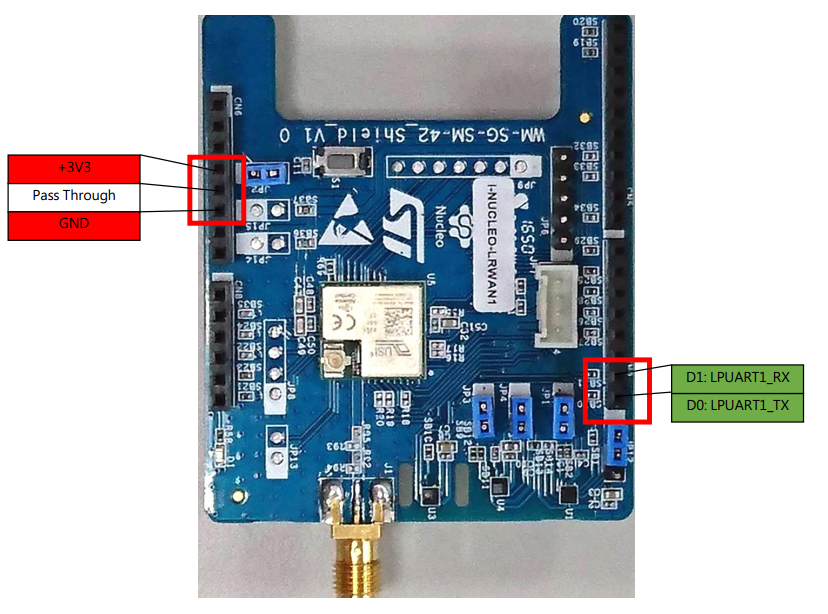
\includegraphics[width=14cm]{source/images/LoRa_mod}
	\caption{I-Nucleo-LRWAN1 \cite{LoRaMod}\label{fig:loraMod}}
\end{figure}

Abbildung \ref{fig:loraMod} zeigt das Endger"at, das zur 
Daten"ubertragung verwendet ist. Diese Platine mit Arduino-Connectoren 
und mehr ist eine integrierte L"osung, die jedem erm"oglicht 
Anwendungen mit der LoRa-Technologie zu entwickeln. Das 
I-Nucleo-LRWAN1 verf"ugt "uber den USI\textregistered\ 
LoRaWAN\texttrademark\ Technologiemodul f"ur kosteng"unstiges und 
stromsparendes Weitverkehrsnetz (LPWAN), welches mit einem 
eingebetteten Stapel von AT-Befehle (AT-Befehl beschreiben) 
mitgeliefert wird. Dieses Board wurde ausgew"ahlt, weil es durch ein 
externes Board wie das Nucleo-L053 oder das B-L475E-IOT01A Discovery 
kit \ref{Node} "uber mehrere Schnittstellen wie \ac{LPUART}, \ac{SPI} 
oder I2C angesteuert werden kann. Noch dazu verf"ugt das 
I-Nucleo-LRWAN1 "uber die folgenden eingebetteten Sensoren.

\begin{itemize}
	\item ST Beschleunigungs- und Magnetosensor (LSM303AGR)
	\item ST relative Feuchtigkeits- und Temperatursensor (HTS221)
	\item ST Drucksensor (LPS22HB)
\end{itemize}

Im Vergleich zu anderen Endger"aten, worauf keine Sensoren vorhanden 
sind, braucht man keine zus"atzliche Sensoren kaufen. Die 
Kommunikation mit einem anderen Mikrocontroller erfolgt einfach durch 
UART, man braucht nicht auf das integrierte Radio-Modul zum Senden oder 
Empfangen von Daten und Befehle zu k"ummern. Das Bild 
\ref{fig:loraMod_intern} zeigt, dass das I-Nucleo-LRWAN1 mit einem 
STM32L0-Mikrocontroller versehen ist, der dazu zust"andig ist, die 
Kommunikation zwischen dem I-Nucleo-LRWAN1 und einem externen 
Mikrocontroller zu vereinfachen. Das SX1272-Chip ist das eigentliche 
LoRa-Radio-Modul, das die Daten oder die AT-Befehle per Funk durch die 
Antenne an entweder einem Gateway oder einem anderen Endger"aten 
sendet. 

\begin{figure}[h]
	\centering
	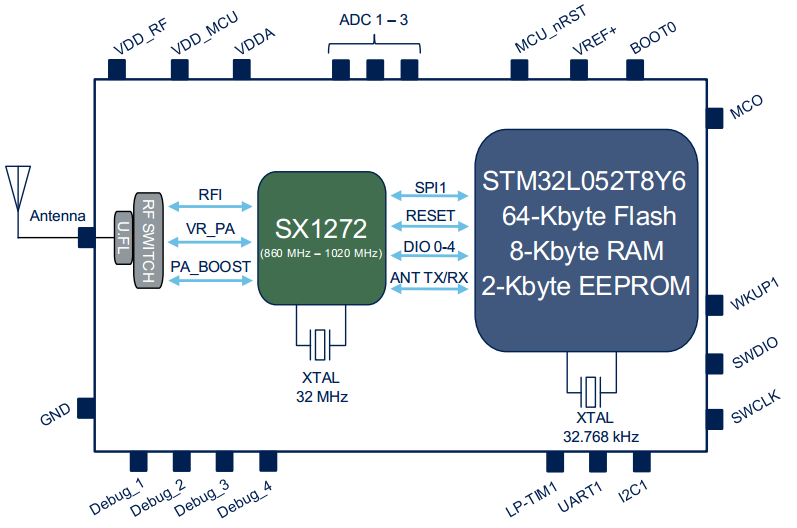
\includegraphics[width=14cm]{source/images/LoRa_Intern}
	\caption{I-Nucleo-LRWAN1 Architektur 
	\cite{LoRaMod}\label{fig:loraMod_intern}}
\end{figure}

\vspace{10cm}
Das I-Nucleo-LRWAN1 wird mithilfe seiner Arduino-Konnectoren mit einem 
externen Board verbunden. F"ur diese Abschlussarbeit wird dieses 
Endger"at an den Arduino-Connectoren des B-L475E-IOT01A Discovery kit 
verbunden (Siehe Abbildung \ref{fig:loranode})

\begin{figure}[h!]
	% first include \usepackage{subfigure}
	\centering
	\subfigure[]{
		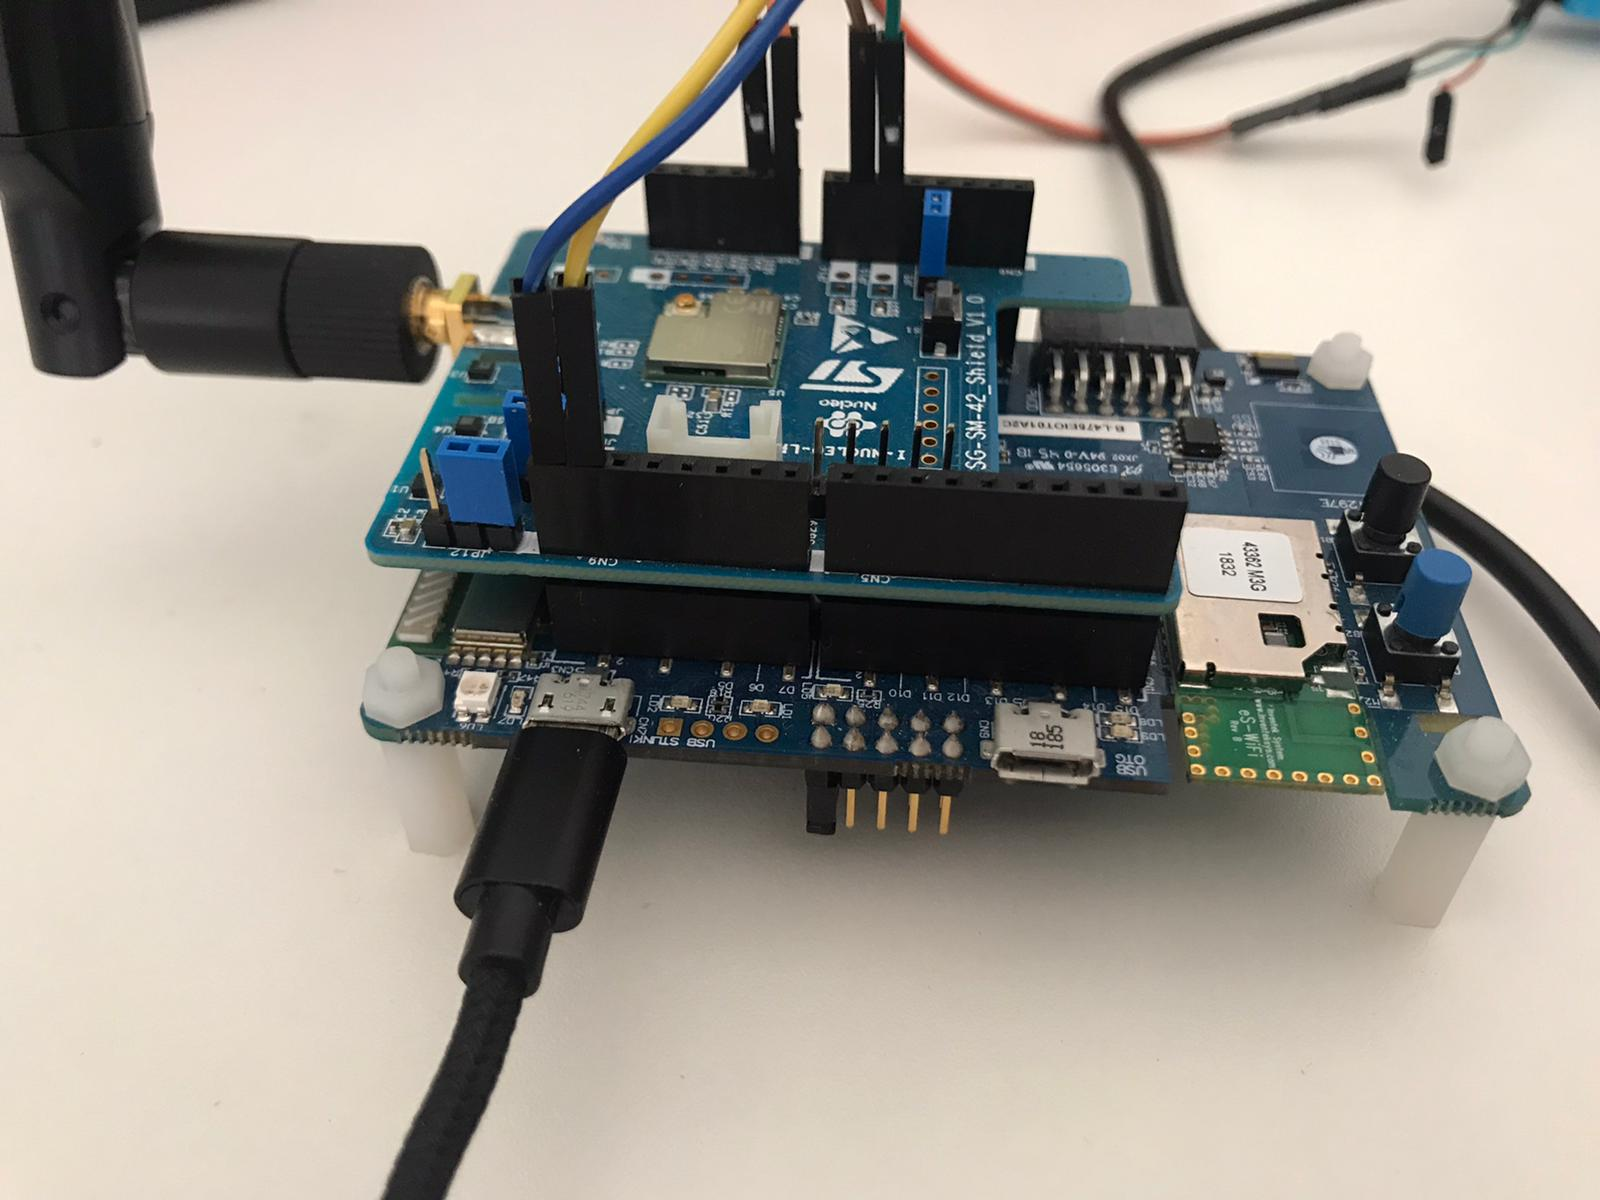
\includegraphics[ width=7cm]{source/images/Node1}
		\label{fig-subfig1}
	}
	\subfigure[]{
		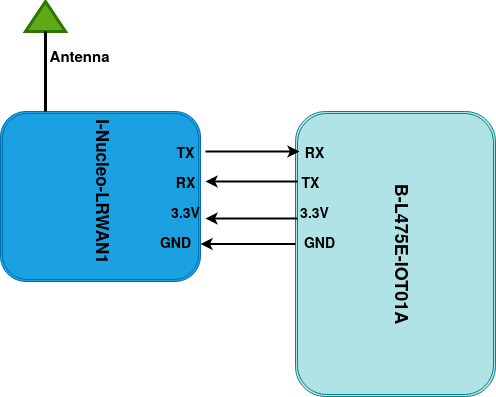
\includegraphics[width=7cm]{source/images/LABCSMARTLoRa-Node}
		\label{fig-subfig2}
	}
	\caption{LABCSMART LoRa End-Node physisches Aussehen 
	\subref{fig-subfig1} und Verbindung 
	\subref{fig-subfig2}\label{fig:loranode}}
\end{figure}

Dem Bild \ref{fig-subfig2} ist zu entnehmen, dass beide Komponenten 
durch eine UART-Schnitt-stelle kommunizieren. Das I-Nucleo-LRWAN1 wird 
von dem  B-L475E-IOT01A mit Strom versorgt. Die Aufgabe des 
B-L475E-IOT01A besteht darin, erstmal die Sensordaten zu verarbeiten, 
als n"achsten sendet es durch die UART-Schnittstelle AT-Befehle zur 
Konfiguration des I-Nucleo-LRWAN1, sodass die erhaltenen Sensordaten 
mithilfe des LoRaWAN-Protokolls gesendet werden. 

\subsection{LoRa und LoRaWAN-Protokol}\label{LoRaWAN_P}

In diesem Teil der Thesis erfahren Sie was LoRa und das 
LoRaWAN-Protokoll sind, als auch wie das Protokoll implementiert wird, 
damit ein Endger"at in dem LoRaWAN-Netzwerk hinzugef"ugt wird.

\subsubsection{LoRa: Die Physikalische Schicht}

Eine einzige Technologie kann nicht alle Anwendungen des IoT 
decken. Technologien wie Wi-Fi und \ac{BLE} sind weit 
verbreitete Standart und decken die Kommunikation pers"onlicher 
Ger"ate recht gut. Die Mobilfunktechnologie passt hervorragend zur 
Anwendung, die einem hohen Datendurchsatz ben"otigen.

Diese Technologien sind zwar gut aber haben es bestehen einige 
Nachteile, wie dem hohen Energieverbrauch und die Strecke von einem 
Sender zu einem Empf"anger ist relativ kurz. LoRa bieten L"osungen zu 
diesen Nachteilen an, n"amlich eine mehrj"arige Batterielebensdauer, 
die "Ubertragung von kleinen Datenmengen "uber gro\ss{}e Entfernungen. 
LoRa ist die physikalische Schicht oder die verwendete drahtlose 
Modulation, um eine lange Bereichskommunikationsverbindung zu 
schaffen. 

Viele "altere drahtlose Systeme verwenden die Frequenzumtastungen
(Englisc \textbf{\textit{\ac{FSK}}}) als physikalishce Schicht, weil es eine sehr 
effiziente Modulkation zur Erzielung geringer Leistung ist. LoRa 
basiert auf die Chirp-Spreizspektrum-Modulation (Englisch 
\textbf{\textit{Chirp Spread Spectrum Modulation}}). Diese Modulation 
beha"alt die gleiche Eigenschaft der geringen Leistung wie 
\ac{FSK}-Modulation bei und erh"oht aber deutlich die 
Kommunikationsreichweite. Das Chirp-Spreizspektrum wird seit 
Jahrzehnten aufgrund seiner Kommunikationsreichweite und seiner 
Robustheit gegen"uber St"orungen in der Milit"ar-und 
Weltraumkommunikation eingesetzt. LoRa ist derzeit die erste 
kosteng"unstige Implementierung f"ur dien kommerziellen Einsatz.

Die LoRa-Technologie wurde von einem kleinen franz"osischen Start-Up 
namens Cycleo entwickelt. In 2012 wurde Cycleo von der Firma Semtech 
gekauft.

Es existiert konkurrierende Technologien zu LoRa  wie Narrowband IoT 
(ND-IoT) und Sigfox. Das LoRa kann  Video- und Audio-Nachrichten nicht 
"ubertragen, man kann nur sehr kleine Datenpakete wie Sensordaten 
"ubertragen. Der Hauptpunkt von LoRa ist die Kommunikation "uber lange 
Strecken und die Verwendung einer sehr geringen Sendeleistung von 
ungef"ahr 20mW. 

Die Reichweite einer LoRA-Kommunikation wird durch ihre Bandbreite, die 
Signalausgangsleistung sowie den verwendeten Spreisfaktor ( Englisch 
\textbf{\textit{\ac{SF}}}) bestimmt. Durch die Steuerung des Signals 
wird seine Reichweite zum Nachteil der Bitrate erh"oht, da es "uber 
einen l"angeren Zeitraum "ubertragen wird. Das verbraucht auch zu viel 
Energie und spielt Nachteilhaft zur Autonomie des Ger"ats. Das hei\ss{}t, 
je gr"o\ss{}er der Spreisfaktor ist, umso kleiner wird die Bitrate und 
die Reichweite wird dagegen gr"o\ss{}er.Ein LoRaWAN-Netzwerk bietet 
sechs m"ogliche Spreizfaktoren (\textbf{SF7, SF8, SF9, SF10, SF11, 
SF12}).  

Die Reichweite zwischen LoRa-Sender und -Empf"anger h"angt von der 
Umgebung ab, in der das Ger"at betrieben wird. Die Abdeckung von 
Innenr"aumen h"angt weitgehend von der Art des verwendeten Baumaterials 
ab. Die Tabelle \ref{tab:Range} zeigt die Reichweite der 
LoRa-Technologie abh"angig der Umgebung.

\begin{center}
	\begin{table}[htbp] 
		\centering 
		\Large
		\begin{tabular}{l|c|r}
			\textbf{Umgebung} & \textbf{Reichweite in kM} \\
			\hline
			St"adtische Gebiete	& 2 bis 5 \\
			\hline
			andische Gebiete & 5 bis 15\\
			\hline
			Direkte Sichtlinie	& >15 
		\end{tabular} 
		\caption{Rechweite abh"angig der Umgebung} 
		\label{tab:Range} 
		
	\end{table}
\end{center}

Es gibt aber Wirtschaftler, die dazu gekommen sind ein Weltrekord zu 
stellen, indem sie eine LoRa-Verbindung bis auf 200Km geschafft haben. 
Ein Beispiel ist Herr Andreas Spiess \cite{AndreasSpiess}.


\vspace{10cm}
\begin{figure}[h]
	\centering
	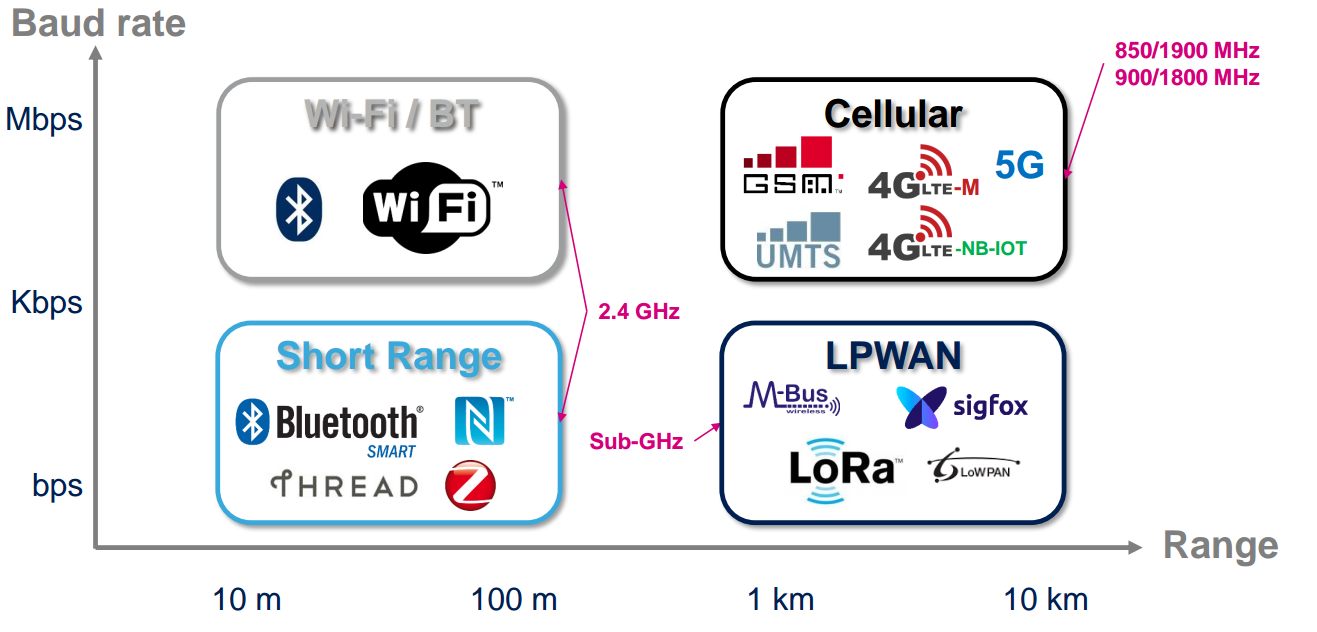
\includegraphics[width=14cm]{source/images/Communications_tech}
	\caption{Vergleich zwischen LoRa und andere IoT 
	Kommunikationstechnologien \cite{LoRaWAN}\label{fig:Netz}}
\end{figure}
Abbildung \ref{fig:Netz} ist zu entnehmen, dass LoRa im Vergleich zu 
andere Technologien wie Wi-Fi oder 4G eine kleine Baudrate hat. Aber 
seine Reichweite ist deutlich gr"o\ss{}er als weit bekannte 
Technologien wie Bluetooth oder Wi-Fi.

Die LoRa-Technologie kann man in vielen Gebiete Einsetzen. Die folgende 
Auflistung gibt einen groben "Uberblick auf einige Einsatzgebiete.

\begin{itemize}
	\item \textbf{Intelligente Dienstprogramme}
	\begin{itemize}
		\item "Uberwachung eines Leistungstransformators
		\item Wasserstands"uberwachung
		\item Kraftstoff"uberwachung
	\end{itemize}

	\item \textbf{Gesundheit und Hygiene}
	\begin{itemize}
		\item Temeratur- und Feuchtigkeits"uberwachung
		\item Umwelt"uberwachung
	\end{itemize}

	\item \textbf{Sicherheit}
	\begin{itemize}
		\item Radioaktivit"ats"uberwachung
		\item Intelligenter Geschwindigkeitsblitzer
	\end{itemize}

	\item \textbf{Landwirtschaft}
	\begin{itemize}
		\item "Uberwachung des Tierschutzes
		\item "Uberwachung der Pflanzenwachstumsbedingungen
	\end{itemize}

		\vspace{3cm}
		\item \textbf{Effizienz}
	\begin{itemize}
		\item Asset Management (Tracking von Containern, Paletten)
		\item Deichmanagement (Verfolgung von Autos, Lieferwagen, 
		Lastwagen)
	\end{itemize}
\end{itemize}

\subsubsection{LoRaWAN: Das Kommunikationsprotokoll}\label{protokol}

LoRaWAN beschreibt das Kommunikationsprotokoll und die 
Systemarchitektur des Netzwerks, w"ahrend LoRa die physikalische 
Schicht, die die Fernkommunikationsverbindung erm"oglicht. Das 
Protokoll und die Netzwerkarchitektur haben den gr"o\ss{}en Einfluss 
auf die Bestimmung der Batterielebensdauer eines Endger"ats, die 
Netzwerkkapazit"at, die Servicequalit"at, die Sicherheit und die 
Vielzahl der vom Netzwerk bereitgesellten Anwendungen. 

\begin{figure}[h]
	\centering
	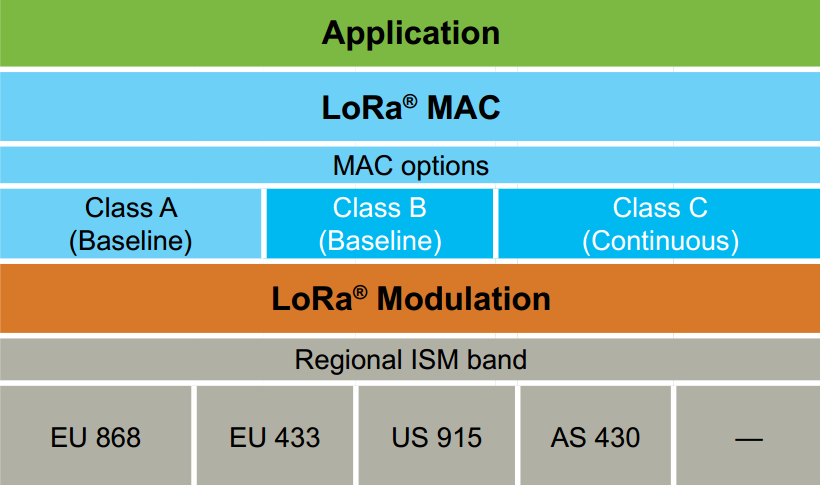
\includegraphics[width=13.5cm]{source/images/LoRa_MAC}
	\caption{Klassen von LoRaWAN \cite{LoRaWAN}\label{fig:LoRaMAC}}
\end{figure}

Wie es auf Abbildung \ref{fig:LoRaMAC} zu entnehmen ist, ist das 
LoRaWAN mit verschiedenen Schichten aufgebaut. Die erste Schicht ist 
die regionale Schicht, hier geht es um die Frequenzbereichen , die 
abh"angig von der Region zur Date"ubertragung verwendet werden k"onnen. 
Die ISM-Bandfrequenzen von Europa liegen zwischen 863 MHz und 870 MHz.
Als n"achstes kommt die LoRa-Modulation als physikalische Schicht des 
Netzwerks. LoRaWAN verf"ugt "uber viele Klassen, n"amlich die Klasse A, 
B und c. Diese Klassen werden sp"ater in diesem Unterkapitel im 
Einzelnen erkl"art. Am Ende kommt die Anwendung der LoRa-Technologie.

Alle Endger"ats funktionieren nicht gleich, dies aufgrund der von dem 
Entwickler implementierte Klasse.

\begin{description}
	\item [Klasse A (All end-devices) \label{classA}]: Ein Endger"at 
	der Klasse A erm"oglich eine bidirektionale Kommunikation, wobei 
	nach jedem Uplink eines Endger"ats f"ur kurze Zeit zwei kurzen 
	Downlink-Empfangsfenstern folgen. Diese Empfangs Fenster werden 
	jeweils f"ur eine Zeit \textit{RECEIVE\_DELAY1}(f"ur das erste 
	Fenster) und \textit{RECEIVE\_DELAY2} ge"offnet. Die Dauer dieser 
	Zeiten werden sowohl in dem Endger"at als auch in dem Server 
	gespeichert. Verglichen zu den anderen Klassen, sind Endger"ate 
	der Klasse A die niedrigsten Leistungsfresser. 
	
	Nachdem die zwei Downlink-Empfangsfenster geschlo\ss{}en sind, kann 
	das Gateway keine weitere Downliks mehr senden. Die n"achsten 
	Downlinks werden erst ber"ucksichtig, wenn das Endger"at ein Uplink 
	gesendet hat.
	Das unten stehende Bild zeigt dieses Verhalten recht gut.
	
	 \begin{figure}[h]
	 	\centering
	 	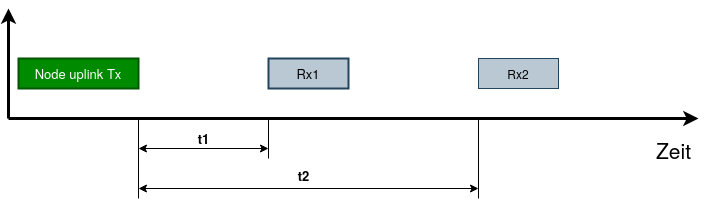
\includegraphics[width=14cm]{source/images/ClassA}
	 	\caption{Klasse A \label{fig:classA}}
	 \end{figure}
	
	\item [Klasse B (Beacon)]: Zus"atzlich zu den zuf"alligen 
	Empf"angsfenster der Klasse A, Ger"ate der Klasse B "offnen 
	zus"atzliche Empfangsfenster zu geplannte Zeiten. Damit das 
	Endger"at seine Empfangsfenster an den geplanten Zeiten "offnen 
	kann, bekommt es  ein synchronisiertes Beacon von dem Gateway. Dies 
	erm"oglicht dem Gateway zu wissen, wann das Endger"at auf Downlinks wartet. Diese Klasse verbraucht mehr Leistung im  Vergleich zur Klasse A. 
	
	 \begin{figure}[h]
		\centering
		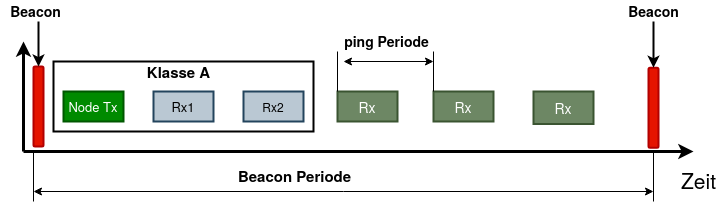
\includegraphics[width=12cm]{source/images/ClassB}
		\caption{Klasse B \label{fig:classB}}
	\end{figure}
	
	\vspace{10cm}
	\item [Klasse C (Continuously listening)]: Endger"ate der Klasse C 
	haben fast immer ge"offnete Empfangsfenster, die sich nur beim 
	Senden schlie\ss{}en. Diese Klasse verbraucht Energie am meisten.
	
	\begin{figure}[h]
		\centering
		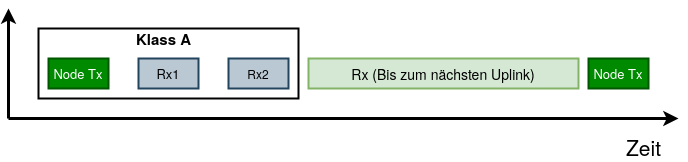
\includegraphics[width=13cm]{source/images/ClassC}
		\caption{Klasse C \label{fig:classC}}
	\end{figure}

\end{description}


Im Rahmen dieser Thesis wird nur die Klasse A ber"ucksichtig, weil das 
ausgew"ahlte Endger"at die Klasse B nicht unterst"utzt und die Klasse C 
zu viel Energie verbraucht. 

\subsection{Sicherung der Daten}\label{secure}

Wir wollen nicht, dass die gesendeten Informationen durch ein Dritter 
ohne Zugriffsrechte auf das Netzwerk die Informationen lesen kann. 
Unabh"angig davon, ob die Netzwerksicherheit oder die Vertraulichkeit 
und Sicherheit der Daten gew"ahrleistet werden soll, ist das Thema 
sicherheit "au\ss{}erst wichtig. Eine Frage, die "ubrigens das 
Internet der Dinge als ganzes betrifft.

Um die Netzwerk- und Datensicherheit zu gew"arleisten, verwendet das 
LoRa-WAN-Netzwerk zwei AES-128-Verschl"usselung. Der erste ist der 
Netzwerksistzungsschl"ussel (Englisch \textbf{\textit{\ac{NwkSKey}}}) 
stellt die Authentizit"at der Ger"ate im Netzwerk sicher. Der zweite 
ist der Anwendungssitzungsschl"ussel (Englisch  
\textbf{\textit{\ac{AppSKey}}}). Der NwkSkey wird von dem 
Endger"at und dem Server benutzt, um den Nachrichtenintegrit"atscode 
(Englisch \textbf{\textit{\ac{MIC}}}) zu berechnen und die Intergit"at 
aller Daten zu pr"ufen.  Es wird weiterhin verwendet, um da  
Nutzdatenfeld von \ac{MAC}-Daten zu verschl"usseln und zu entschl"usseln. 

Der AppSKey wird auch vom Endger"at und Server verwendet diesmal, um 
das Nutzdatenfeld von anwendungsspezifische Daten zu verschl"usseln 
und zu entschl"usseln. Die anwendungsnutzdaten werden zwischen dem 
Endger"at und dem Anwendungsserver Ende-zu-Ende verschl"usselt. Das 
hei\ss{}t der Netzwerkserver kann m"oglicherweise den Inhalt der 
"ubertragene Daten "andern. 

\begin{figure}[h]
	\centering
	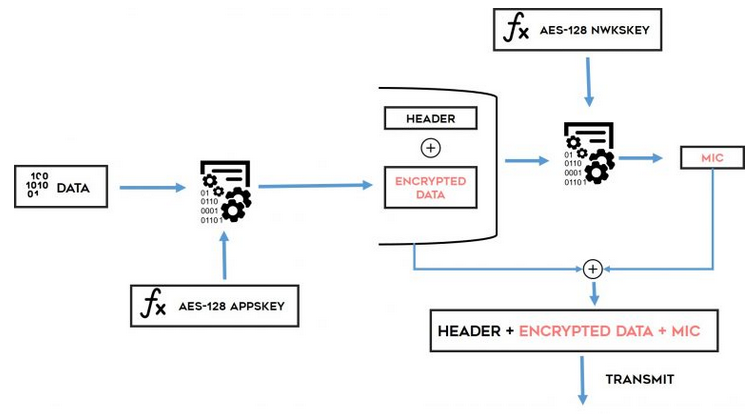
\includegraphics[width=14cm]{source/images/WAN}
	\caption{LoRaWAN-Nachricht Verschl"usselung 
		\cite{Entcription}\label{fig:Entcription}}
\end{figure}

Laut Abbildung \ref{fig:Entcription} werden die zu sendende Daten erst 
mit dem AppSKey verschl"usselt. Ein Header, der andere Adressen des 
Endger"at enth"alt, wird an den verschl"usselten Daten hinzugef"ugt. 
Nach dieser Verkn"upfung wird das MIC berechnet, der nach der 
Berechnung an den verschl"usselten Daten und dem Header hinzugef"ugt 
wird. Nun k"onnen die Daten versandt werden. 

Nachdem der Server die Daten empfangen hat, kann die Integrit"at 
dieser Daten vom Server mithilfe des MICs gepr"uft werden. Die Daten 
werden nur ber"ucksichtigt, wenn das MIC stimmt, ansonsten werden sie 
verworfen.  

\vspace{5cm}
\subsection{Aktivierung des Endger"ats}
Damit ein Endger"at dem LoRaWAN-Netzwerk hinzugef"ugt werden kann, 
muss es erst spezifiziert und aktiviert werden. Die Aktivierung eines 
Endger"at kann auf zwei Arten erfolgen, entweder per 
Over-The-Air-Aktivierung (Englisch \textbf{\textit{\ac{OTAA}}}), oder 
per Aktivierung durch Personalisierung (Englisch 
\textbf{\textit{\ac{ABP}}}), wobei die zwei Schritte der 
Personalisierung und Aktivierung in einem Schritt erfolgt. 

\subsubsection{Aktivierung durch OTAA}
Damit die Over-The-Air-Aktivierung vollst"andig wird, m"ussen 
Endger"ate zwe-cks Datenaustausch mit einem Server einem Join-Verfahren 
folgen. Dieses Verfahren wird auch durchgef"uhrt, wenn es vorkommen 
w"urde, dass ein Endger"at die Sitzungsinformationen verloren hat.
Bevor ein Endger"at das Join-Verfahren startet, muss er folgende 
Informationen haben: Ein eine global eindeutige Endger"atekennung 
(\textbf{DevEUI}), eine Anwendungskennung (\textbf{AppEUI}) und ein 
AES-128-Schl"ussel (\textbf{AppKey}). 


\begin{description}
	\item[AppEUI:] ist 8-Byte-Wert, codiert in Hexadezimalformat und 
	bezeichnet eine Kennung des Anwendungsanbieter.
	\item[DevEUI:] ist ein 8-Byte-Wert mit hexadezimaler Codierung und 
	bezeichnet die eindeutige Kennung eines Endger"ats. Manche 
	LoRa-Radiomodule beinhalten eine DevEUI vom Herstellung her. Wenn 
	nicht schon vorhanden, diese kann vom Anwendungsanbieter gesetzt 
	werden.
	\item[AppKey:] ist ein 16-Byte-Wert in Hexadezimalformat.Wenn ein 
	Endge"at mit OTAA das Netzwerk beitritt, wird dieser Schl"ussel zur 
	Herstellung des NwkSKey und des AppSKey verwendet, um die 
	Netzwerkkommunikation und die Anwendungsdaten zu verschl"usseln und 
	zu pr"ufen. 
\end{description}

Sobald das Endger"at mit diesen Informationen versehen ist, kann es eine 
Join-Abfrage (\textbf{Join request}) am Server schicken. Der Server 
antwortet mit einem Join-Zustimmung (\textbf{Join accept}), wenn das 
Endger"at dem Netzwerk beitreten darf. Die Join-Accept- Nachricht wird 
wie ein normales Downlink gesendet aber benutzt zwei unterschiedliche 
Verz"ogerungen verglichen mit \textit{RECEIVE\_DE-LAY1} und 
\textit{RECEIVE\_DELAY2} der im Abschnitt \ref{classA} beschriebenen 
Verz"ogerungen. Diese Verz"ogerungen sind \textit{JOIN\_ACCEPT-\_DELAY1} 
und \textit{JOIN\_ACCEPT-\_DELAY2}. Dem Endger"at wird keine Antwort 
geschickt, wenn die Join-Abfrage abgelehnt wurde.

Die Join-Accept-Nachricht enth"alt ein 3-Byte-Anwendung Nonce 
(\textit{AppNonce}), eine Netzwerkkennung (\textit{NetID}), eine 
Endger"atadresse (\textit{DevAddr}), eine Verz"ogerung zwischen TX und 
RX (\textit{RxDelay}) und eine optionale Liste der Kanalfrequenz 
(\textit{CFList}). Die DevAddr und das AppNonce sind die wichtigste 
Informationen bei einer Join-Accept-Nachricht.

\begin{description}
	\item[DevAddr:] ist eine 4-Byte-Adresse, womit der Server und das 
	Endger"at nach Aktivierung kommunizieren.   
	
	\item[AppNonce:] ist ein zuf"alliger Wert, die vom Netzwekserver 
	bereitgestellt wird und vom 
	Endger"at verwendet, um den NwkSkey und den AppSKey abzuleiten.
	Der NwkSkey und der AppSKey werden mit der internen Funktion   
	\textbf{\textit{aes128\_encrypt}} (im LoRa-Radiomodule vom 
	Hersteller zur Verf"ugung gestellt) und wird wie folgt bestimmt 
	\cite{LoRaWAN}:
	
	\textbf{NwkSKey = aes128\_encrypt(AppKey,0x01 \textbar AppNonce 
	\textbar NetID \textbar DevNonce \textbar pad)
	NwkSKey = aes128\_encrypt(AppKey,0x02 \textbar AppNonce \textbar 
	NetID \textbar DevNonce \textbar pad)} 
\end{description}

Nun k"onnen Endger"ate, die dem Neztwerk beigetreten sind, Informationen 
mit dem Netzwerkserver austauschen (Uplinks und Downlinks). Abbildung 
\ref{fig:request} beschreibt das oben erl"auterte Verfahren.


\begin{figure}[h]
	\centering
	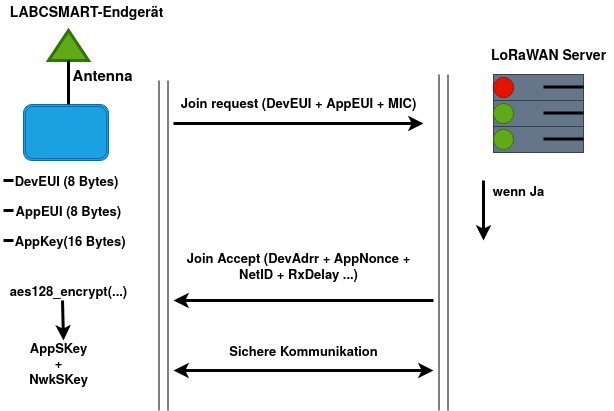
\includegraphics[width=14cm]{source/images/Join-Procedure}
	\caption{Join-Request Verfahren\label{fig:request}}
\end{figure}


\vspace{10cm}
\subsubsection{Aktivierung durch ABP}

Bei dieser Aktivierungsart, braucht das Endger"at keine Join-Abfrage 
senden, hier geht es um, eine direkte Bindung eines Endger"at zu einem 
bestimmten Netzwerk. Das bedeutet, dass die \textit{DevAddr} und die 
zwei Sitzungsschl"ussel (\textit{AppSKey} und \textit{NwkSKey}) an 
Stelle der \textit{DevEUI}, \textit{AppEUI} und \textit{AppKey}, im 
Endger"at gespeichert werde. Jedes Endger"at soll einen eindeutigen Satz 
von \textit{AppSKey} und \textit{NwkSKey}. Das Kompromittieren der 
Schl"ussel eines Ger"ats sollte die Sicherheit der Kommunikation anderer 
Ger"ate nicht beeintr"achtigen. 


Zusammengefasst ist OTAA komplexer als ABP aber bietet eine h"ohere 
Sicherheit. Falls ein Prototyp oder ein kleines Netzwerk erstellt werden 
soll, ist ABD genug. Wenn es um ein gr"o\ss{}ers Netzwerk geht, ist OTAA 
empfohlen, weil es sicherer und agiler ist. 

\vspace{5cm}
\subsection{AT Kommandos}\label{AT}

Nun wissen wir was LoRa und LoRaWAN sind und wie es funktioniert, aber 
nicht wie Informationen (Appkey, NwkKey und mehr) dem Endger"at 
zugewiesen werden als auch wie die Daten am Server gesendet werden. 
Im Kapitel \ref{LoRa Modul} wurde das Wort ``AT-Befehl'' kurz erw"ahnt, 
in diesem Abschnitt erfahren Sie was diese Befehle sind und welche 
gebraucht werden, damit die eine Verbindung per OTAA oder per ABP 
erfolgreich wird.

Im UNIX-Systemen ist AT ein Kommando, das bewirkt, das andere Kommandos
nur einmal ausgef"uhrt werden. Hier ist es benutzt, um das
i-nucleo-lrwan1 einzustellen. Da das LoRa-Radiomodul sich nicht selbst
einstellen kann, ist auch die Aufgabe des B-L475E-IOT01A \ref{Node} die 
Einstellung durchzuf"uhren. Das i-nucleo-lrwan1 verf"ugt "uber eine 
UART-Schnittstelle (Siehe \ref{fig:loraMod}), um mit dem B-L475E-IOT01A 
zu komunizieren. Diese UART-Schnittstelle hat folgende 
Konsolenkonfiguration: 

\begin{itemize}
	\item Baudrate: 115200
	\item Daten: 8 Bit
	\item Parit"at: keine
	\item Stopbit: 1 Bit
\end{itemize}           

Die Syntax des Kommandos ist wie folgt: 
 
 \begin{itemize}
 	\item Algemeine Kommandos: 
 	\begin{itemize}
 		\item \textbf{AT:} Pr"uft ob die UART Schnittstelle benutzbar ist
 		\item \textbf{ATE [=<enable>]:}  Aktivieren oder Deaktivieren
 		des lokalen Echos
 		\item \textbf{ATZ:} Modul zur"ucksetzen
 		\item \textbf{AT+VERB [=<enable>]:} Ausführliche Antwort
 		aktivieren oder deaktivieren 
 	\end{itemize}
 	\item LoRa MAC-Kommandos: \textbf{AT+Kommando [=parameter]}
 	Die MAC-Komm-andos werden hier nicht alle dargestellt, da es zu lang
 	w"are sie alle zu erkl"aren. Zur Erkl"arung aller Kommandos siehe
 	das AT-Befehlsreferenzhand-buch \cite{AT_Command}.
 	Die Zeichnen [ ] bedeuten, dass der Parameter optional ist. Mit
 	Parametern ist ein AT-Befehl wie ein Set-Befehl, und ohne ist es ein
 	Get-Befehl.
 \end{itemize}  

Da wir nun wiessen, wir diese Kommandos zu nutzen sind, k"onnen wir 
Beispiele f"ur OTAA und ABP machen (Diese Einstellungen wurden getestet
und funktionieren einwandfrei).

\begin{itemize}\label{LoRaconf}
	\item[\textbf{OTAA:}] Die Folgenden AT-Befehle weden von
	B-L475E-IOT01A nacheinander  per UART am i-nucleo-lrwan1 gesendet.
	\begin{itemize}
		\item \textbf{AT+BAND=0}: Setzt die Region des Netzwerks (Hier
		EU868)
		\item \textbf{AT+CLASS=0}: Die Klasse A wird verwendet 
		\item \textbf{AT+DC=1}: Deaktiviert den Auslastungsgrad 
		\item \textbf{AT+DR=0}: Setzt die TX-Datenrate (LoRa SF12/125KHz
		250 Bit/s)
		\item \textbf{AT+RX2DR=0}: Setzt die TX-Datenrate (LoRa
		SF12/125KHz 250 Bit/s)
		\item \textbf{AT+RX1DT=1000}: Setzt die Verz"ogerung des ersten
		Enpfangsfenster (in ms)
		\item \textbf{AT+RX2DT=2000}: Setzt die Verz"ogerung des zweiten
		Enpfangsfenster (in ms)
		\item \textbf{AT+JRX1DT=5000}: Setzt die Verz"ogerung des
		zweiten Enpfangsfenster (in ms)
		\item \textbf{AT+JRX2DT=6000}: Setzt die Verz"ogerung des
		zweiten Enpfangsfenster (in ms)
		\item \textbf{AT+RF=14,8671000000,12,0,1}: Konfiguriert das
		LoRa-Radiomodule. Ausgansleistung: 14dBm, Frequenz: 867.1MHz,
		Spreading factor: SF12, Bandbreit: 125KHz, Cyclic Codingrate:
		4/5.  
		\item \textbf{AT+APPEUI=ABC123ADF135CBD8}: Setzt die AppEUI
		\item \textbf{AT+AK=00112233445566778899AABBCCDDEEFF}: Setzt den
		AppKey 
		\item \textbf{AT+JOIN=1}: Sendet eine Join-Abfrage als OTAA
		 
	\end{itemize}
	
	\item[\textbf{ABP:}] Die Folgenden AT-Befehle weden von
	B-L475E-IOT01A nacheinander  per UART am i-nucleo-lrwan1 gesendet.
	\begin{itemize}
		\item \textbf{AT+BAND=0}
		\item \textbf{AT+CLASS=0} 
		\item \textbf{AT+DC=1}
		\item \textbf{AT+DR=0} 
		\item \textbf{AT+RX2DR=0}
		\item \textbf{AT+RX1DT=1000} 
		\item \textbf{AT+RX2DT=2000} 
		\item \textbf{AT+JRX1DT=5000}
		\item \textbf{AT+JRX2DT=6000} 
		\item \textbf{AT+RF=14,8671000000,12,0,1}
		\item \textbf{AT+ADDR=12345678}: Setzt die Ger"atadresse 
		\item \textbf{AT+NSK=1122334455663EAB546829CB361CAB7D}: Setzt
		den NwkSKey
		\item \textbf{AT+ASK=887766554433BCFACDE52476CA4598BA}: Setzt
		den AppSKey 
		\item \textbf{AT+JOIN=0}: Sendet eine Join-Abfrage als ABP
	\end{itemize}

	\item[\textbf{Daten senden}:] \textbf{AT+SEND=2,Daten,1}
	Hier werden die Daten durch das Port 2 gesendet. Die Daten mussen in
	hexadezimaler Format sein, und sollen nicht gr"o\ss{}er als 64 Bytes
	sein. Die 1 am Ende steht f"ur die Best"atigung des Datenempfangs. 
	
\end{itemize}

Im AT-Befehlsreferenzhandbuch stellt das Appendix 3 Tabellen f"ur die
Konfiguration der Datenrate abh"angig von der Region zur Verf"ugung.

\chapter{Gateway und LoRaWAN-Server}\label{G_S}

Nun ist es m"oglich ein Endger"at, so einzustellen, dass es f"ahig ist,
Uplinks an einem LoRaWAN-Server zu senden und Downlink vom Server zu
bekommen. Aber was ist das LoRaWAN-Server und wozu wird das Gateway
benutzt. Diese Fragen werden in diesem Kapitel beantwortet.

\section{Gateway}\label{Gateway}

Es gibt fertige Gateways auf dem Markt, die man kaufen und direkt
einsetzen kann . F"ur diese Thesis wird ein selbst gebautes Gateway
benutzt. Der Grund daf"ur ist das es billiger als fertige Gateway ist,
sich ein eigenes zu bauen. Noch dazu steckt eine wissenschaftliche Idee
dahinter. Zu wissen, wie ein Gateway gebaut wird, welche Komponenten
und welche Software im Spiel kommen.  

Ein Gateway ist ein Ger"at, das aus mindestens einem Konzentrator, einem
Host und einer Netzverbindung zum Internet oder ein privates Netzwerk
(Ethernet, 3G, Wi-Fi), m"oglicherweise einem GPS-Empf"anger besteht. Der
Konzentrator ist ein Board, das Funkpakete senden und empfangen kann.
Ein Konzentrator basiert auf einem Semtech-Mehrkanalmodem
(\textbf{\textit{SX130x}}), einem Transceiver (\textbf{\textit{SX135x}})
und/oder eigenst"andige Modems mit geringem Stromverbrauch
(\textbf{\textit{SX127x}}).  

Ein Host ist ein eingebetteter Computer, auf dem die Paketweiterleitung
ausgef"urt wird. Der Host steuert den Konzentrator "uber eine
SPI-Schnittstelle. F"ur diese Arbeit ist der Host ein Raspberry-Pi. Ein
Gateway kann viele Endger"ate gleichzeitig behandeln. Die Kommunikation
zwischen einem Endger"at und einem Gateway ist bidirektional, das hei\ss{}t
das Endger"at sendet dem Gateway Daten, aber kann auch Daten von dem
Gateway empfangen.

Die Kommunikation von einem Endger"at zum Gateway ist ein Uplink,
w"ahrend die Kommunikation vom Gateway zum Endger"at ein Downlink ist.
Ein Endger"at sendet Uplinks als Broadcast, das hei\ss{}t die gesendeten
Daten werden von allen Gateways des Netzwerks bekommen. Das Gateway
leitet das Datenpaket an dem Netzwerkserver weiter. Der Netzwerkserver
sammelt die Nachrichten aller Gateways, filtert doppelte Daten heraus
und bestimmt das Gateway mit der besten Rezeption. Der Netzwerkserver
leitet seine Daten zu dem entsprechenden Anwendungsserver, womit der
Nutzer die Sensordaten ansehen und/oder verarbeiten kann.

Bekommt den Netzwerkserver eine Antwort vom Anwendungsserver, bestimmt
der Netzwerkserver welches Gateway benutzt wird, um dem Endger"at die
Antwort zu senden (Downlink).

Der Konzentrator kann Funktpakete zwar empfangen und senden, er ist
aber nur eine elektronische Komponente und braucht eigentlich eine
Software, um empfangene oder zu sendenden Pakete zu bearbeiten. Diese 
Software hei\ss{}t LoRa-Packet-Forwarder \cite{paketForwarder}. 
Der Paket-Forwarder ist ein Programm, das auf dem Host ausgef"uhrt wird,
um Funkpakete, die vom Konzentrator empfangen werden "uber eine IP/UDP-
Verbindung an den Server weiterleitet und sendet die vom Server gesendeten 
Funkpakete weiter. Der Packet-Forwarder kann auch ein netzwerkweites
synchrones GPS-Signal senden, das zur Koordination aller Endger"ate des
Netzwerks verwendet wird. 


\begin{figure}[h!]
	% first include \usepackage{subfigure}
	\centering
	\subfigure[]{
		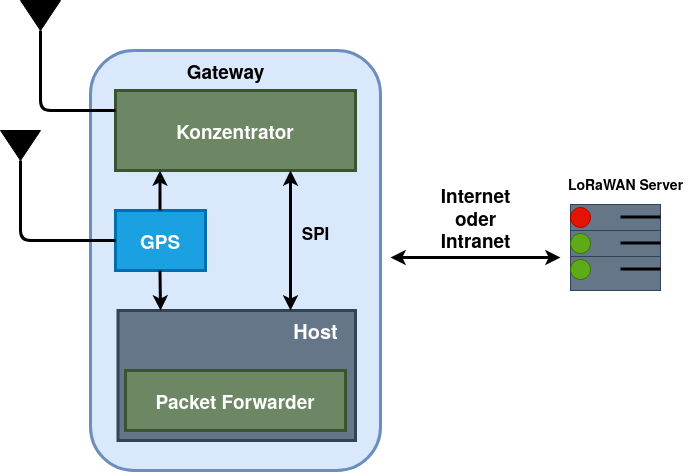
\includegraphics[ width=8cm]{source/images/LoRa_gateway}
		\label{fig:forwarder1}
	}
	\subfigure[]{
		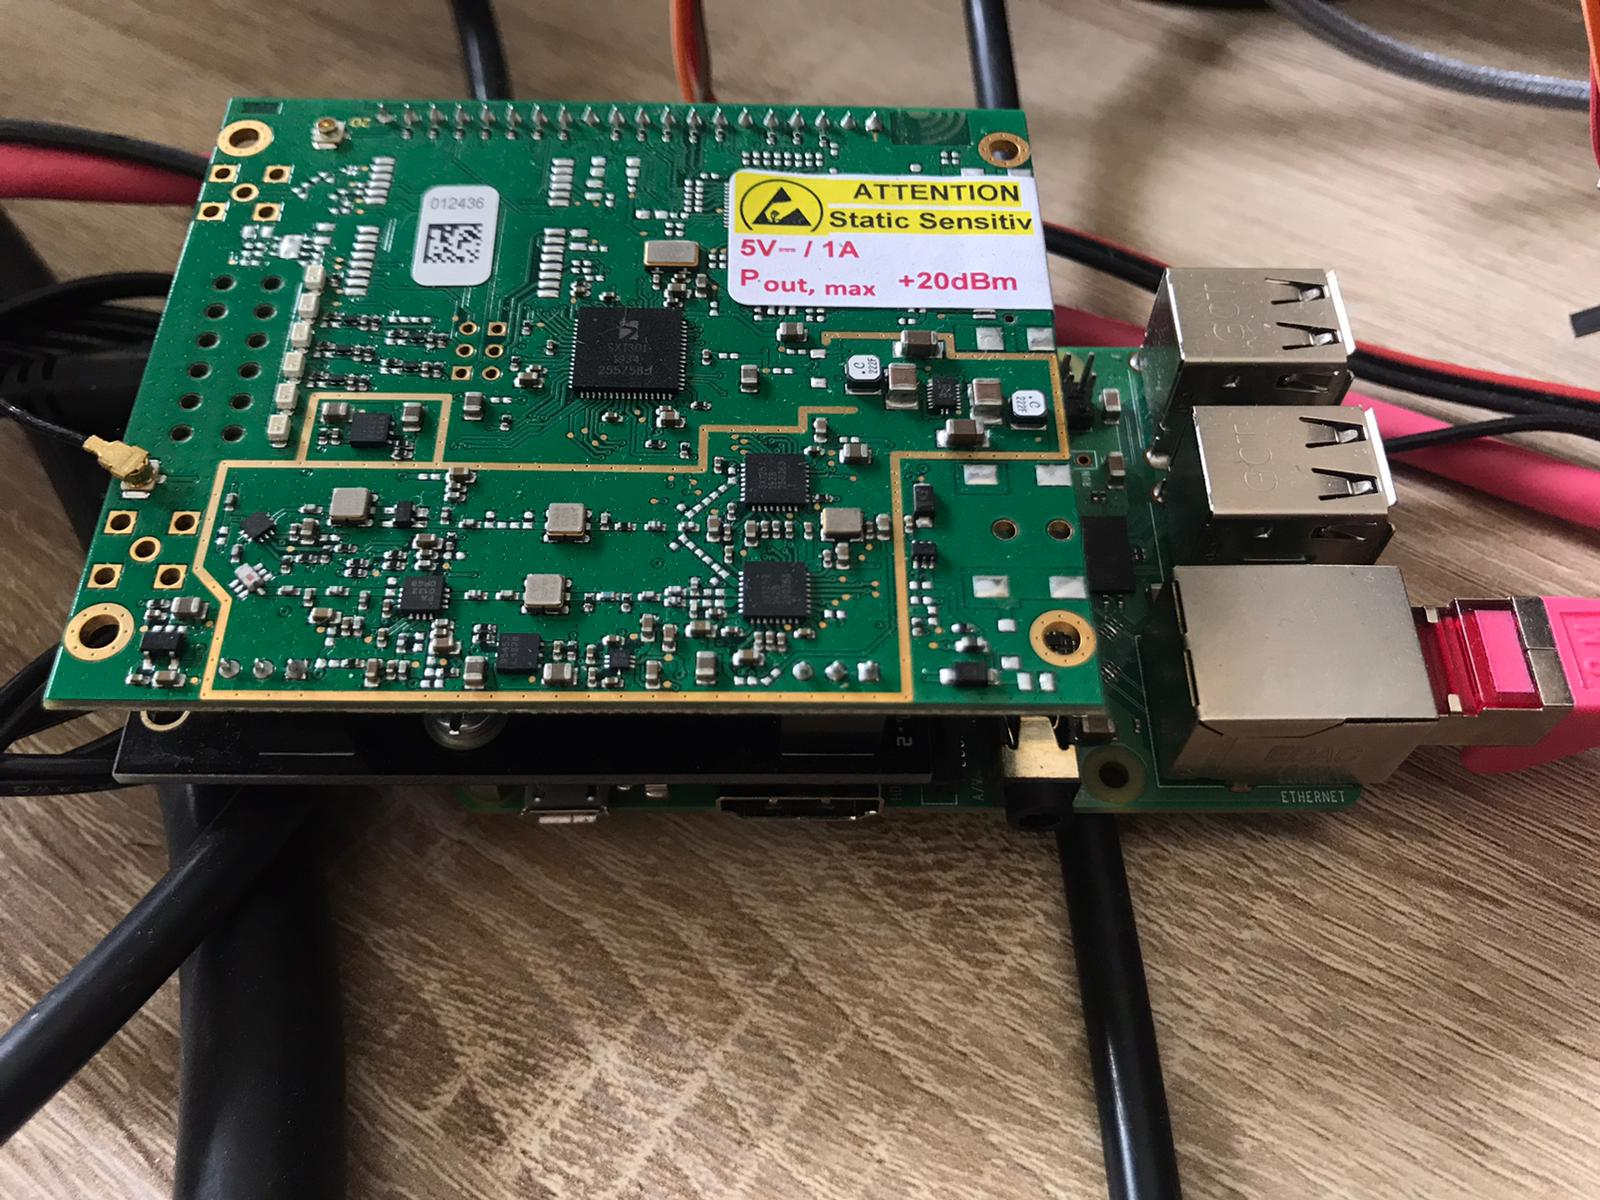
\includegraphics[width=6cm]{source/images/Gateway2}
		\label{fig:forwarder2}
	}
	\caption{LABCSMART LoRaWAN Gateway}
\end{figure}


Abbildung \ref{fig:forwarder1} zeigt die Netzwerkkomponenten, beginnend
mit dem Gateway und seinen Bestandteilen. Es ist deutlich zu sehen, dass
das der Konzentrator und der Host durch einer SPI-Schnittstelle verbunden
sind und die Verbindung zwischen dem Gateway und dem Server das Internet
einem einzigen Modul. Das hei\ss{}t, der Konzentrator, das Gateway und der
Server zusammen in einem Block eingebaut sind. Der Raspberry-Pi ist
gleichzeitig der Host und der Server. 

\section{Einstellung des LoRaWAN-Servers}\label{server}

An dieser Stelle ist die Arbeit fast fertig, da unsere Anwendung
theoretisch in der Lage ist, Uplinks an dem Gateway zu schicken. Nun
interessieren wir uns auf die Verarbeitung der empfangenen Daten. Die
Daten werden zwar in die Luft gesendet, aber der Benutzer kann diese
nicht sehen oder verarbeiten, dazu ist ein Server. Dieser Server soll in
der Lage sein, gesendete Funkpakete zu interpretieren und darzustellen,
sodass der Benutzer diese lesen und verstehen kann. 

Der verwendete Server hei\ss{}t \textbf{lorawan-server} (Open-source). Er
wurde von Herrn \textbf{Petr Gotthard} \cite{server} entwickelt und ist
ein Kompakter Server f"ur private LoRaWAN-Netzwerke. Dieser Server dient
nicht nur als Netzwerkserver, sondern auch als Anwendungsserver. Man kann
damit alle Ereignisse, und alle Daten, die entweder vom Endger"at oder
vom Packet-Forwarder kommen. Der Server wurde in 79\% in der
Programmiersprache Erlang \cite{erlang} geschieben.   

In diesem Kapitel, erfahren Sie wie dieser Server einzustellen ist, um
Endger"ate mit OTAA oder ABP zu verbinden. Bevor ein Endger"at
hinzugef"ugt wird, muss der Server dazu vorbereitet werden. Er muss die
MAC-Adresse des Gateways, der Netzwerk, das Profil des Netzwerks und die
Gruppe des Endger"ats kennen. 


\begin{description}
	\item[Gateway:] Der Server kann mit einem oder mehrere Gateways
	verbunden werden (Nur ein in unserem Fall). Der Server bekommt alle
	Uplinks, die von den Gateways weitergeleitet werden, betrachtet nicht
	welches Endger"at welchem Netzwerk geh"ort.
	\vspace{10cm}
	\begin{figure}[h]
		\centering
		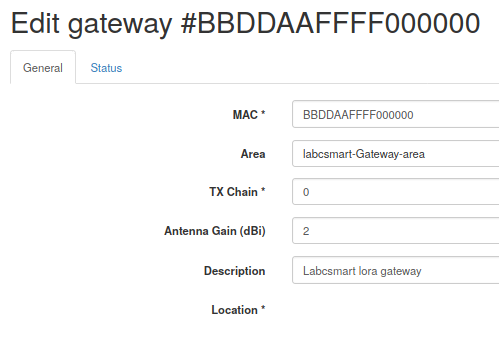
\includegraphics[width=8cm]{source/images/Gateway}
		\caption{Einstellung des Gateways\label{fig:gateway}}
	\end{figure}

	\item[Netzwerk:] Der Server kann ein oder mehrere Netzwerke
	 verarbeiten. Jede Netzwerkkonfiguration umfasst:
	\begin{itemize}
		\item Eine Netzwerkkennung, um die Enger"at-Adresse (DevAddr) neu
		verbundener Endger"ate zu Erstellen.
		\item LoRaWAN-Regionparameter, einschlie\ss{}lich zus"atzliche
		Frequenzen
	\end{itemize}

	\begin{figure}[h!]
		% first include \usepackage{subfigure}
		\centering
		\subfigure[]{
			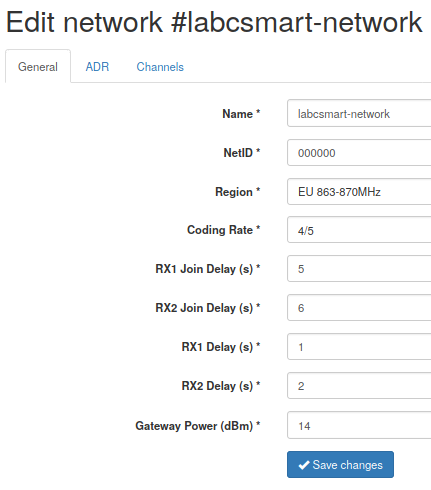
\includegraphics[
			width=7cm]{source/images/Labcsmart_network_gen}
			\label{fig:NetGen}
		}
		\subfigure[]{
			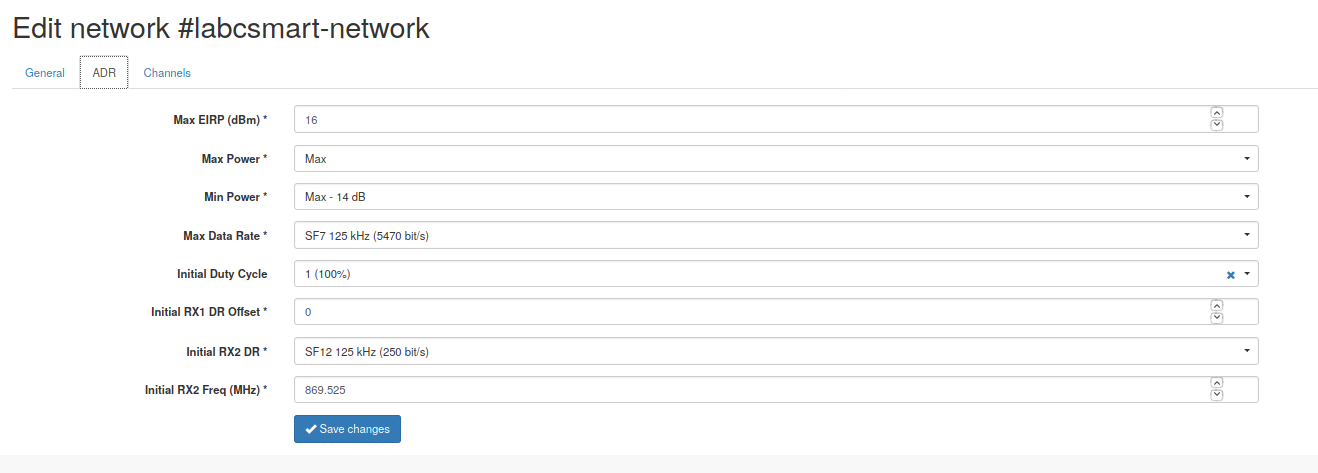
\includegraphics[width=7cm]{source/images/Labcsmart_network_adr}
			\label{fig:NetAdr}
		}
		\caption{Einstellung des Netzwerks}
	\end{figure}


	
	\item[Profil:] Das Profil repr"asentiert eine bestimmte Hardware und
	alle statischen Einstellungen in der Firmware, die f"ur eine Gruppe
	von Ger"aten gleich sind. Die Konfiguration umfasst:
	\begin{itemize}
		\item Die Referenz zu einem bestimmten Netzwerk
		\item Die F"ahigkei des Ger"ats, \ac{ADR} 
		durchzuf"uren oder den Batteriestatus bereitzustellen.
		\item Die Anwendung
	\end{itemize} 
	Es ist zu bemerken, dass die Einstellung der Abbildung
	\ref{fig:ProAdr} genau ist, wie die Einstellung des Endger"ats, die
	im Abschnitt \ref{LoRaconf} erl"autert wurde. Weil wir genau dieses
	Ger"at im Netzwerk integrieren wollen, muss auch der Server
	dem entsprechen eingestellt werden.

	\begin{figure}[h!]
		% first include \usepackage{subfigure}
		\centering
		\subfigure[]{
			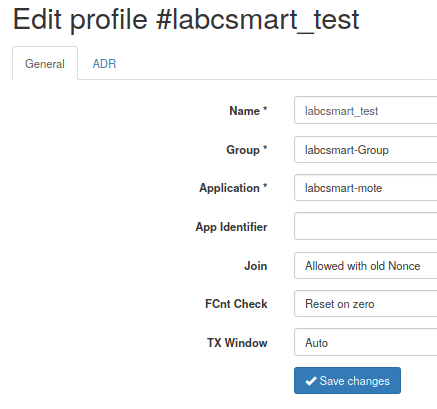
\includegraphics[
			width=7cm]{source/images/Labcsmart_profile_gen}
			\label{fig:ProGen}
		}
		\subfigure[]{
			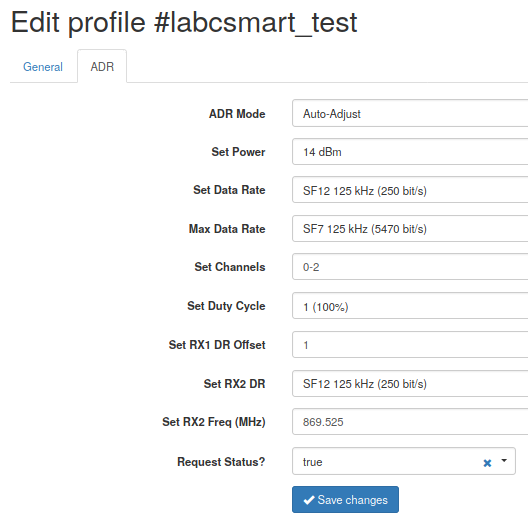
\includegraphics[width=7cm]{source/images/Labcsmart_profile_adr}
			\label{fig:ProAdr}
		}
		\caption{Einstellung des Profils}
	\end{figure}
	
	\item[Gruppe:] Die Gruppe repr"asentiert eine Reihe von Profilen,
	die zu einem einzelnen Teilnetzwerk geh"oren. Zu einem einzelnen
	Kunde zum Beispiel.
	\begin{figure}[h]
		\centering
		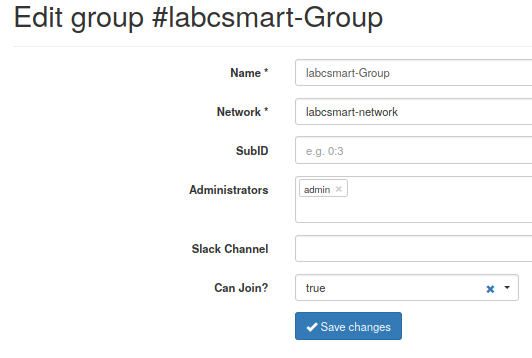
\includegraphics[width=10cm]{source/images/Labcsmart_group}
		\caption{Einstellung der Gruppe\label{fig:group}}
	\end{figure}
\end{description}
\vspace{10cm}
Nun ist es m"oglich Endger"ate zum Server hinzuzuf"ugen. Als Erstes
versuchen wir mit ABP, dann mit OTAA.

\subsubsection{ABP Verbindung}
Ger"ate die mit ABP verbunden werden sollen, brauchen wir im Abschnitt
\ref{secure} DevAddr, NwkSKey und AppSKey.
Die Informationen auf Abbildung \ref{fig:DevAdr} werden automatisch
erstellt, nachdem ein Endger"at dem Netzwerk hinzugef"ugt wurde. Man
kann die "Ubertragungsfrequenzen, die Leistung und andere Einstellungen
erkennen, die im Abschnitt \ref{secure} erw"ahnt wurden. 
	\begin{figure}[h!]
	% first include \usepackage{subfigure}
	\centering
	\subfigure[]{
		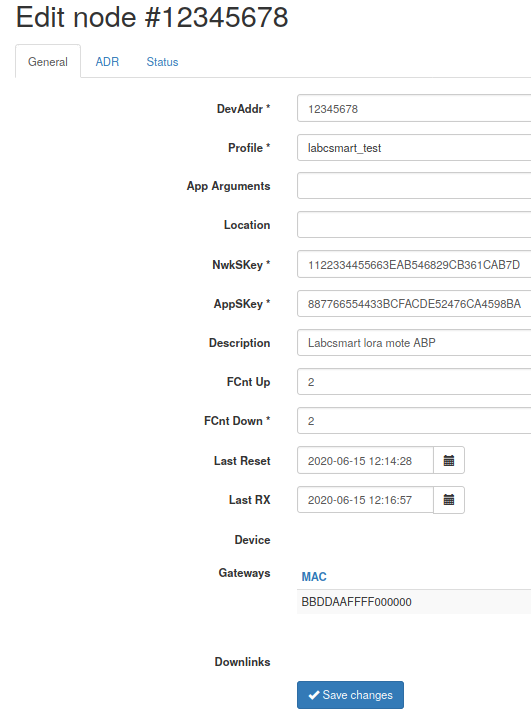
\includegraphics[ width=7cm]{source/images/Labcsmart_abp_gen}
		\label{fig:DevGen}
	}
	\subfigure[]{
		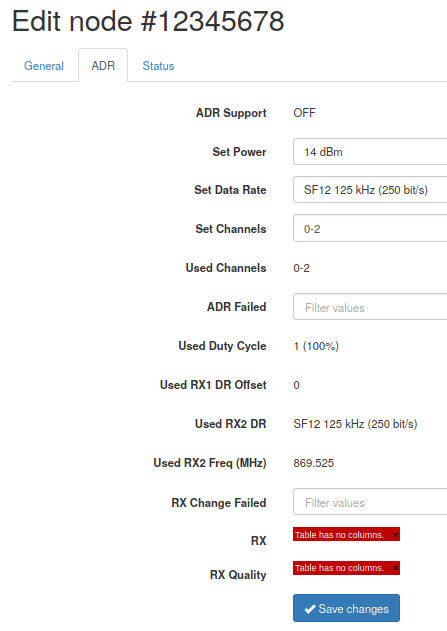
\includegraphics[width=7cm]{source/images/Labcsmart_abp_adr}
		\label{fig:DevAdr}
	}
	\caption{ABP Verbindung}
	\end{figure}

\vspace{10cm}
\subsubsection{OTAA Verbindung}
Hier befinden sich Ger"ate, die dem LoRaWAN-Netzwerk mitmilfe von OTAA
beitreten d"urfen. Man muss dazu aber die DevEUI, AppEUI und AppKey auf
jedem Fall kennen und im Server eingeben (Siehe \ref{fig:otaa}). 
	\begin{figure}[h]
	\centering
	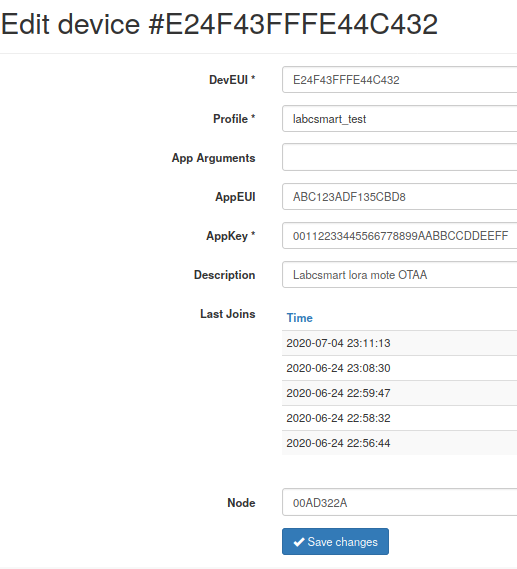
\includegraphics[width=10cm]{source/images/Labcsmart_otaa_gen}
	\caption{Einstellung OTAA\label{fig:otaa}}
\end{figure}
Nachdem das Ger"at dem Netzwerk beigetreten ist, bekommt es eine
DevAddr, einen NwkSKey und einen AppSKey, die mit Hilfe des AppKey
berechnet wird (Siehe \ref{secure} f"ur die Erkl"arung). 
\vspace{10cm}

Nachdem diese Einstellungen fertig sind und die Ger"ate dem Netzwerk
beigetreten sind, k"onnen Uplinks im Dashboard gesehen werden. Der
Inhalt (In Hexadezimal) befinden sich unter Frames (unten links vom
Server). 

	\begin{figure}[h!]
	% first include \usepackage{subfigure}
	
	\subfigure[]{
		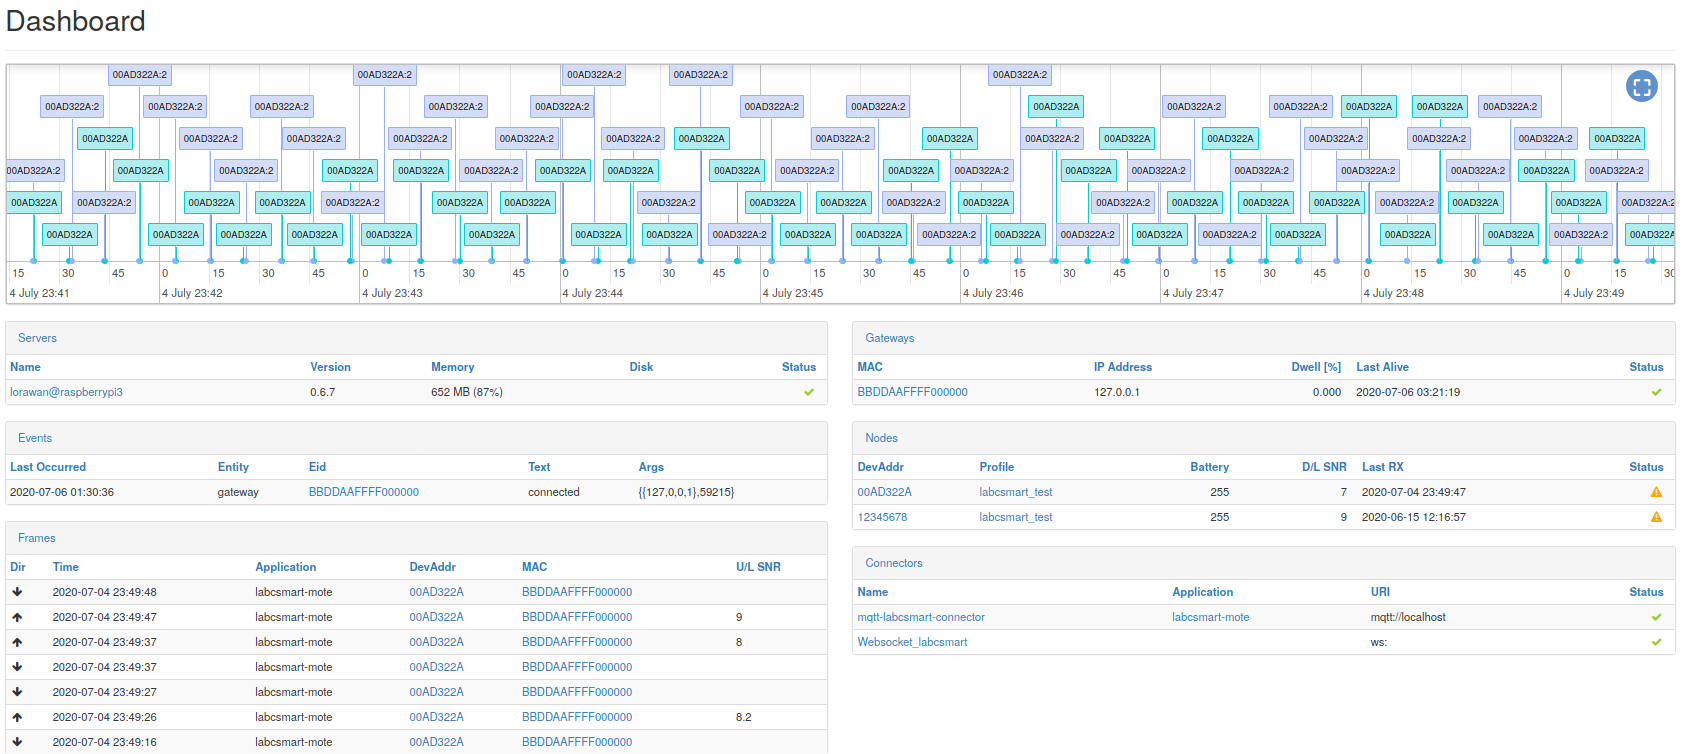
\includegraphics[ width=17cm]{source/images/dashboard}
		\label{fig:Dashboard}
	}
	\subfigure[]{
		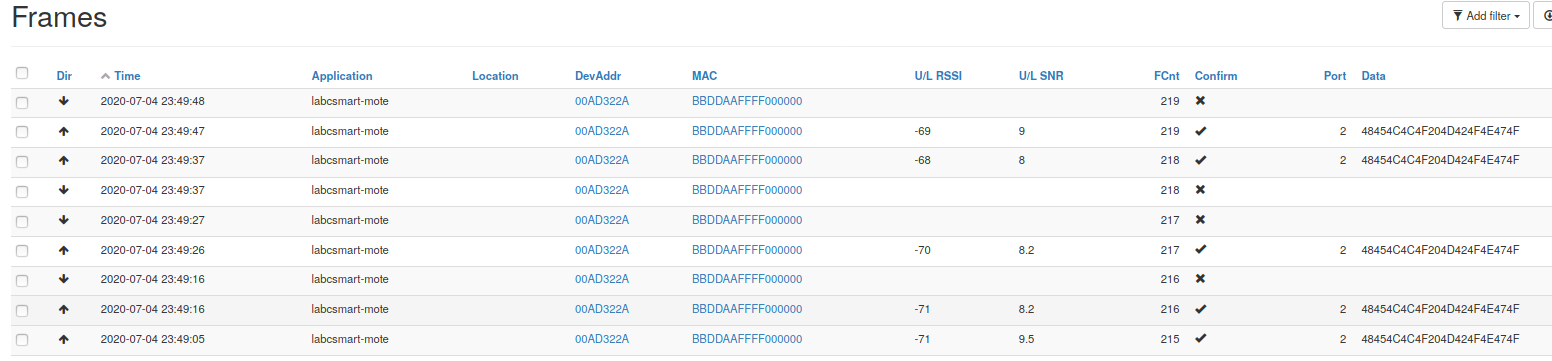
\includegraphics[width=17cm]{source/images/frames}
		\label{fig:Frames}
	}
	\caption{Zwischenergebnis}
\end{figure}

\vspace{10cm}
Gr"une Ereignisse im Abbildung \ref{fig:Dashboard} bezeichnen 
Downlinks, w"ahrend Ereignisse in lila sind Uplinks. Die Spalte U/l 
RSSI des Abbildungs \ref{fig:Frames} stellt die empfangene 
Signalat"arke (Englisch \textbf{\textit{\ac{RSSI}}}) dar. RSSI ist die 
empfangene Leistung in milliwatts, wird aber in \ac{dBm} gemessen. 
Diesen wird sagt wie, gut ein Empf"anger gesendete Signale empfangen 
kann. RSSI ist ein negativer Wert, je n"aher 0 dieser Wert ist, desto 
besser ist das Signal. Der minimale RSSI-Wert f"ur die 
LoRa-Technologie ist -120dBm.  

Zu Ende reicht dieses Ergebnis noch nicht. Was passiert, wenn der Server
nicht mehr funktioniert? Soll die Anwendung auch nicht funktionieren
oder gibt es eine andere M"oglichkeit die Daten irgendwie zu sichern,
falls ein Serverausfall vorkommen w"urde? Zwischen dem Server und dem
Packet-Forwarder gibt es ein Kommunikationsprotokoll namens \ac{MQTT}. 

Das n"achste Kapitel erkl"art was MQTT ist, wie es funktioniert und 
wie die Daten beim Serverausfall anderswo gesichert werden k"onnen. 
  
\section{MQTT Protokoll}

MQTT hat sich in den letzten Jahren zum Standard Protokoll f"ur die
Machine-To-Machine- und IoT-Kommunikation von Ger"ate und Anwendungen
entwickelt. MQTT steht f"ur \textbf{Message Queue Telemetry Transport},
und bietet eine sichere, versl"assliche, performante und wartbare
Kommunikation zwischen Anwendungen und Ger"ate. Dieses Protokoll
unterscheidet sich von Request/Resp-onse-Protokollen wie \ac{HTTP} 
dadurch, dass es alle Kommunikationsteilnehmer entkoppelt. F"ur den
Datenaustausch werden Nachrichten "uber einen zentralen Verteiler an 
die Teilnehmer gesendet. Das ist der Grund warum kein tieferes Wissen 
"uber empfangende Anwendungen vorhanden sein muss.

MQTT basiert auf eine 1:N-Kommunikation, ein Teilnehmer sendet eine
Nachricht, worauf einen oder mehreren Abonnenten Zugriff haben k"onnen.
Teilnehmer k"onnen entweder Date empfangen oder senden. Der MQTT-Broker
ist der zentraler Verteiler, "uber den alle Kommunikationen stattfinden.
Der Publisher ist produziert die Nachricht und der Subsriber abonniert
sich an eine bestimmte oder an alle Nachrichten. 

Der Begriff  Topic, bezeichnet ein Ordner oder Unterordner, an dem
Nachrichten ver"offentlicht oder empfangen werden k"onnen. M"ochte ein
MQTT-Subscriber Nachrichten f"ur ein Topic empfangen, abonniert er es
beim MQTT-Broker. Ein Abonnement kann direkt f"ur ein konkretes Topic
erfolgen, oder es k"onnen Teilb"aume der Topic-Hierarchie abonniert
werden. Die abonnierten Subscriber werden durch den Broker vom
Vorhandensein neuer Nachrichten benachrichtigt, statt selbst beim 
Server "Anderungen anzufragen. Subscriber und Publisher bleiben "uber 
eine \ac{TCP}-Verbindung mit dem MQTT-Broker verbunden. Diese 
Verbindung wird von den Clients (Subscriber und Publisher) selbst 
aufgebaut und ben"otigen anders als der Broker keine Ip-Adresse. 

Kommen wir nun zur"uck auf den Zusammenhang zwischen MQTT und dieser
Thesis. Das Das Kommunikationsprotokoll zwischen dem Packet-Forwarder und 
dem LoRaWAN-Server wurde im Kapitel \ref{server} nicht erw"ahnt. Beide
benutzen das MQTT-Protokoll, um jeweils Uplinks und Downlinks
weiterzuleiten. Es ist derzeit m"oglich mit einer Externen Anwendung an
den vom MQTT-Broker ver"offentlichte Topics zu abonnieren als auch 
selber ver"ofentlichen. Die von der externen Anwendung ver"offentliche 
Topics k"onnen Downlinks ersetzen, diesmal werden die Downlinks nicht 
vom Server gesendet, sondern von der Externen Anwendung.

\chapter{Software Emplimmentierung}\label{Soft-Ent}
Bis jetzt wurden die Begriffe theoretisch erw"ahnt. Man kann zwar schon 
verstehen, was das Ziel der Arbeit ist, wie die gemessenen Daten gelesen 
werden und wie die LoRa funktioniert. Das reicht aber noch nicht. 
In diesem Kapitel geht es um den Host (der Entwicklungsrechner), die 
Tools, die zur Entwicklung der eingebetteten Software zur Ansteuerung 
der Sensoren und des LoRa-Moduls eingesetzt wurden. Das gesamte Projekt 
wurde zum gr"o\ss{}ten Teil in der Programmiersprache C geschrieben. 
Die externe Anwendung f"ur das Abonnieren an Topics und das Senden von
Downlinks wurde in der Programmiersprache Python geschrieben.

\section{Entwicklungsumgebung}
Das gesamte Projekt wurde unter Ubuntu durchgef"uhrt. Ubuntu ist eine 
ber"umte Linux-Distribution. Da die Kosten der Entwicklung niedrig wie 
m"oglich gehalten werden sollen, wurde eine Linux. Distribution 
ausgew"ahlt. Der Grund daf"ur ist die Freiheit von Linux, und die 
Unentgeltlichkeit vieler Entwicklungsumgebung. 

\subsection{Eclipse}

Als Entwicklungsumgebung war \textbf{Eclipse} vorteilhaft, weil der 
Entwickler viele externen Tools hinzuf"ugen kann und es sich einfach 
zum Bedarf angepasst werden kann. In diesem Teil des Berichts, wird in 
die Installation und die Konfiguration von Eclipse eingegangen, sodass  
der Entwickler C-Quelle-Codes durch einen Klick compilieren und im 
Mikrocontroller laden kann. 

\vspace{2cm}
Starten wir erstmal mit der Installation der Entwicklungsumgebung. 
Folgende Kommandos sorgen daf"ur:

\begin{lstlisting}[frame=single]
	$ sudo apt update
	$ sudo apt install oracle-java8-installer
	$ sudo apt install oracle-java8-set-default
\end{lstlisting}

Man soll nun Eclipse von der offiziellen
\href{https://www.eclipse.org/downloads/}{Website}  herunterladen.Nachdem 
die Software heruntergeladen wurde, befindet sie sich unter 
~/Download. Die Software soll entpackt werden bevor die Installation 
erfolgt.
\begin{lstlisting}[frame=single]
	$ tar xfz ~/Downloads/eclipse-inst-linux64.tar.gz
	$ ~/Downloads/eclipse-installer/eclipse-inst
\end{lstlisting}

Die Software startet, es wird nach dem Paket gefragt, die man 
installieren m"ochte. F"ur diese Arbeit brauchen wir das Paket 
\textbf{Eclipse IDE for C/C++ Developers}. Nachdem es ausgew"ahlt 
wurde, kann man nun die Installation starten.
  
Nach der Installation kann man Eclipse eigentlich schon benutzen. 
C-Quelle-Codes f"ur normalen Rechner k"onnen kompiliert werden, da der 
GCC-Compiler standartm"a\ss{}ig installiert wird. Wir wollen aber 
C-Codes f"ur einen ARM-Mikro- controller compilieren. Aus diesem Grund 
m"ussen wir ein externes Tool f"ur ARM-Mikrocontroller in Eclipse 
einf"ugen. Damit das erfolgt, soll man das 
\textbf{Eclipse-Marketplace} 
unter \textbf{Help} suchen. Sobald das Eclipse-Marketplace ge"offnet 
ist, soll man nach \textbf{GNU MCU Eclipse} suchen und 
installieren.

Nun k"onnen wir ein Projekt herstellen. Bevor das geschieht, soll man 
ein Ordner herstelle, in dem das Projekt abgelegt wird. In diesem 
Ordner muss man ein MAKEFILE herstellen. Folgende Kommandos zeigen wie 
das geht.
\begin{lstlisting}[frame=single]
$ mkdir projekt1
$ cd projekt1
$ touch Makefile
\end{lstlisting}
Die Datei ist momentan leer und wird sp"ater ausgef"ullt. Danach w"ahlt
man \textbf{file -> new -> project} aus. Nun wird nach dem Typ des 
Projekts, wir w"ahlen \textbf{Makefile Project with Existing Code} und 
dann \textbf{ARM Cross GCC} aus. Oben gibt man den Namen  sowie das
Verzeichnis des Projekts ein und dr"uckt auf fertig. Nun ist unser 
Projekt angelegt, obwohl wir noch keinen ARM-Code compilieren k"onnen.

Wir wollen mithilfe von \textbf{MAKEFILES} unsere Quellen-Codes 
kompilieren. Wir haben dadurch eine volle Kontrolle auf die 
Kompilierung haben, und die Fehlerausgaben werden schnell 
verst"andlich, da wir genau bekommen was wir auch in dem MAKEFILE 
spezifiziert haben. Wir m"ussen dazu sogenannte \textbf{Build Targets} 
hinzuf"ugen. 

Oben rechts von Eclipse befinden sich diese Build-Targets und m"ussen wie in Abbildung \ref{fig:build} konfiguriert werden.

\begin{figure}[h]
	\centering
	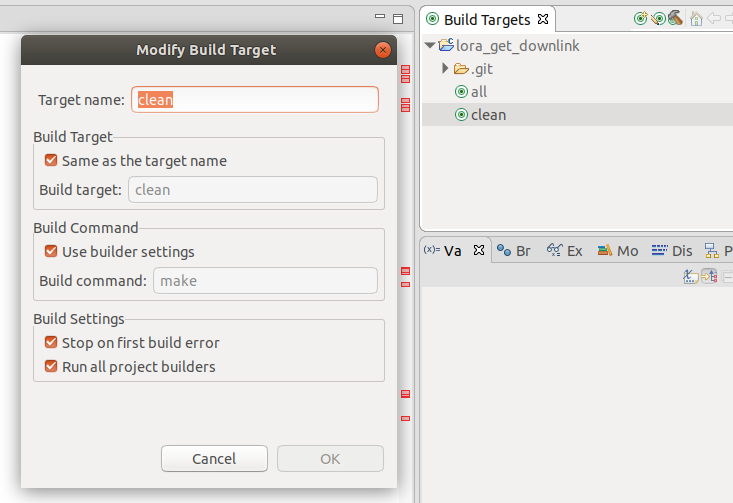
\includegraphics[width=13cm]{source/images/Build}
	\caption{Build Targets einstellen\label{fig:build}}
\end{figure}

Nachdem die Build-Targets konfiguriert sind, erscheinen sie in dem 
\textbf{Project Explorer} wie es der Abbildung \ref{fig:build2} zu 
entnehmen ist. Zum Kompilieren soll man 2 mal auf \textbf{all} klicken, 
genau so wie auf \textbf{clean}, wenn Bin"ar- und ausf"hrbare Dateien 
gel"oscht werden sollen. 

\begin{figure}[h]
	\centering
	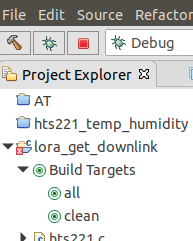
\includegraphics[width=4cm]{source/images/Build2}
	\caption{Build Targets fertig\label{fig:build2}}
\end{figure}

 \vspace{1cm}
\begin{lstlisting}[frame=single]
PROJECT = lora_get_downlink //Name des Projekts
BUILD_DIR = bin //Verzeichnis der gebildete Dateien

CFILES = main.c //C-Quelle-Codes die Kompiliert werden muessen
CFILES += lora_modul.c
CFILES += lsm6dsl.c
CFILES += setup.c
CFILES += hts221.c
CFILES += systick.c

DEVICE=stm32l475vg //Der benutzte Mikrocontroller

LDSCRIPT = ./stm32-clicker.ld //Der Linker
LDFLAGS += -u _printf_float //Damit floating points durch UART dastellbar werden

VPATH += $(SHARED_DIR)
INCLUDES += $(patsubst %,-I%, . $(SHARED_DIR))
OPENCM3_DIR=../libopencm3 //Das Verzeichnis der benutzte Bibliotek

include $(OPENCM3_DIR)/mk/genlink-config.mk
include ./rules.mk
include $(OPENCM3_DIR)/mk/genlink-rules.mk

\end{lstlisting}
Der oben stehenden Textblock ist der Inhalt, der dem Makefile geh"oren 
muss, damit die Kompilierung erfolgt.
 
\textbf{Bemerkung:} Man kann das gleiche Makefile bei neuen Projekten 
benutzen, aber der Name des Projekts, der Mikrocontroller und die zu 
kompilierenden C-Quelle-Dateien  m"ussen je nach Aufgabe angepasst 
werden.   

Damit der kompilierte Code auf dem Mikrocontroller getestet werden kann, muss er in dem Flash-Speicher gespeichert werden. Daf"ur brauch man ein zus"atzliches Werkzeug. Dieses Werkzeug hei\ss{}t \textbf{ST-Link} f"ur STM32-Mikrocontroller. Dieses Werkzeug wird wie folgt installiert.

\begin{lstlisting}[frame=single]
sudo apt-get install libusb-1.0-0-dev git
git clone https://github.com/texane/stlink stlink.git
cd stlink.git
make
\end{lstlisting}
Nun ist das Programm installiert aber man kann es nicht einfach und "uberall ausf"uren. Damit es m"oglich wird, das Programm unter irgendwelchen Ordner und ohne SUDO-Rechte auszuf"uhren, muss es in dem Linux-Filesystem kopiert werden.
\begin{lstlisting}[frame=single]
cd flash
sudo cp st-flash /usr/bin
cd ..
sudo cp *.rules /etc/udev/rules.d
sudo restart udev
\end{lstlisting}

Nehmen wir an, das der kompilierte Code \textbf{stlinkTest.bin} hei\ss{}t. Das Board mit dem STM32L4-Mikrocontroller soll mit dem Entwicklungsrechner durch ein USB-Kabel  verbunden werden. Jetzt kann man den Code mit ST-Link in dem Mikrocontroller speichern. 
\begin{lstlisting}[frame=single]
st-flash write stlinkTest.bin 0x8000000
\end{lstlisting}

\subsection{Libopencm3 Bibliotek installieren}
Sensoren, die f"ur dieses Projekt eingesetzt wurden lassen sich durch 
eine I2C-Schnittstelle ansteuern, w"ahrend die UART-Schnittstelle f"ur 
das Senden von AT-Befehlen verwendet wurde. Wir k"onnen zwar diese 
Peripherien durch direkter Zugriff auf Registern, aber das w"urde zu 
viel Zeit nehmen, und der Code kann un"ubersichtlich werden. Damit wir 
uns diese Arbeit ein wenig sparen, wurde eine Open-Source-Bibliothek 
benutzt \textbf{(libopencm3)} \cite{lib}. 

Diese Bibliothek stellt fertige Funktionen und Parameter zur 
Ansteuerung der Peripherien der ganzen 
ARM-Cortex-M3-Mikrocontroller-Familie zur Verf"ugung. 
Es gibt in dem GNU-ARM-Tool von Eclipse eine Bibliotek f"ur ARM-Mikrocontroller.
Diese wurde nicht verwenden, weil sie zu dem Makefile nicht 
passen w"urde, und die Dokumentation nicht gefunden wurde. 

Libopencm3 verf"ugt "uber eine Doxygen-Dokumentation, die man mit 
einem Browser aufrufen kann. Man muss diese Bibliothek erstmal 
herunterladen bevor die Dokumentation verf"ugbar wird. Folgende
Kommandos zeigen, wie das geht.

\vspace{5cm}

\begin{lstlisting}[frame=single]
/* Bibliothek herunterladen und bilden */
$ git clone https://github.com/libopencm3/libopencm3 
$ make

/* Beispiele */
$ git clone https://github.com/libopencm3/libopencm3-examples 
$ make

/* Dokumentation bilden */
$ cd libopencm3/doc/ 
$ make 

\end{lstlisting}

Nach der Installation kann die Dokumentation mithilfe eines 
Internetbrowser ge"offnet werden (Siehe Abbildung \ref{fig:Lib}).
\begin{lstlisting}[frame=single]
$ firefox index.html 
\end{lstlisting}

\begin{figure}[h]
	\centering
	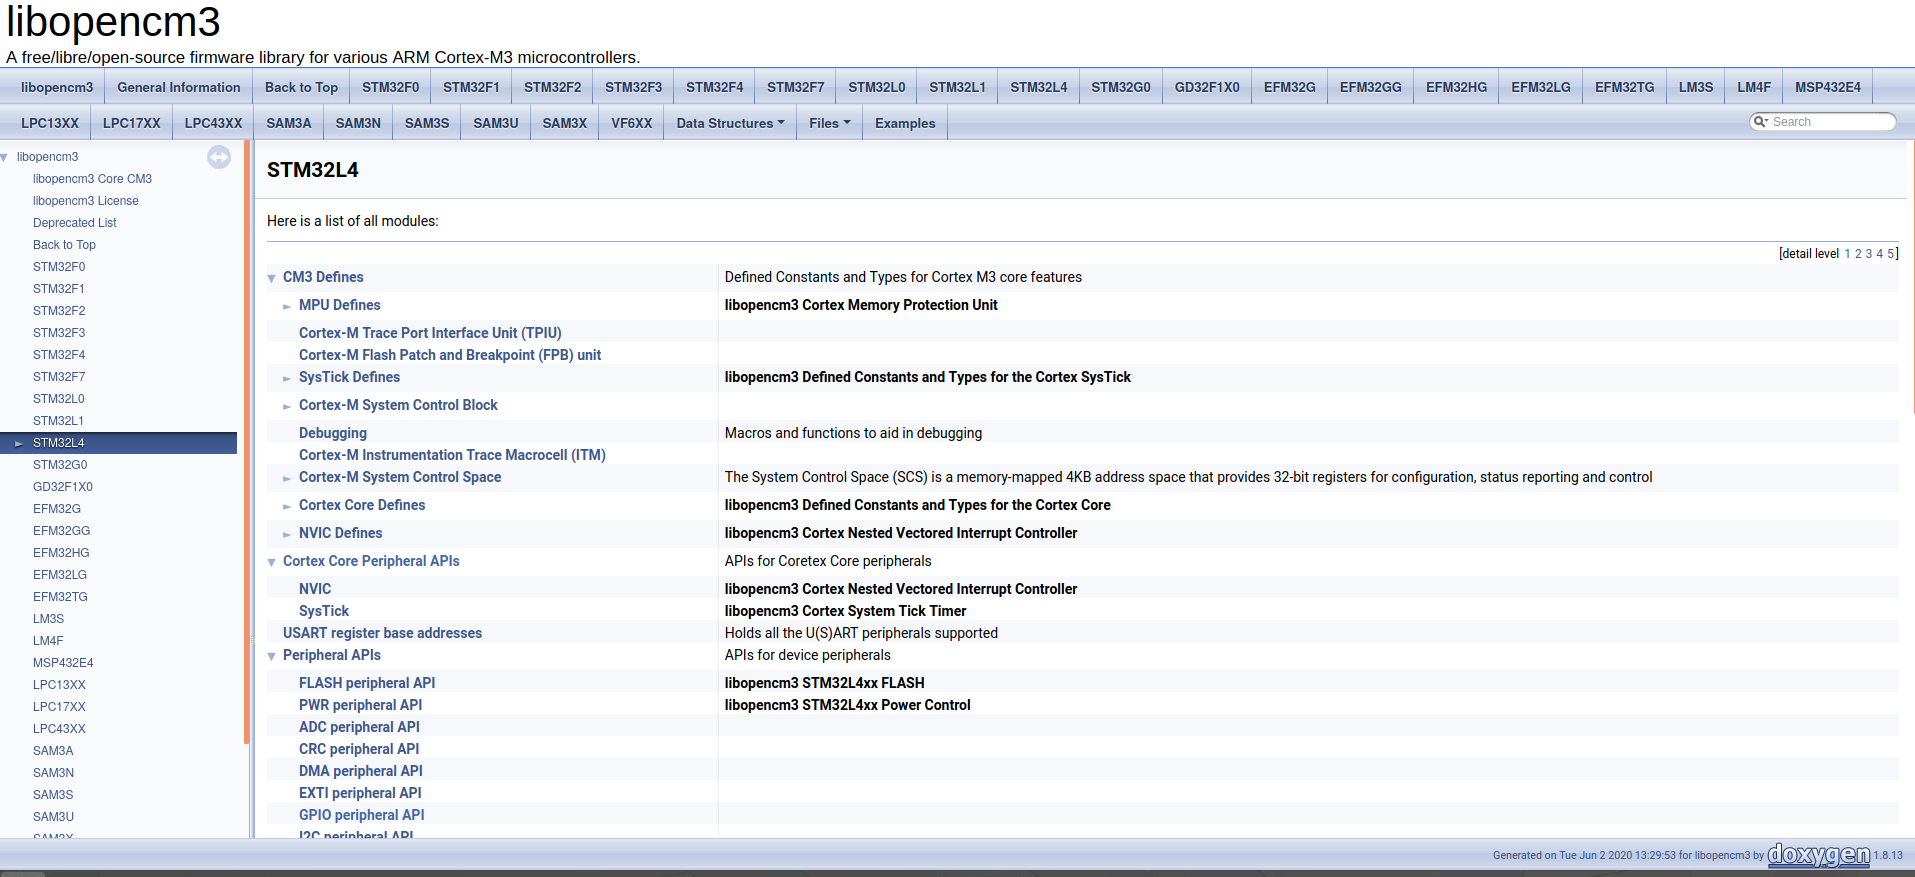
\includegraphics[width=16cm]{source/images/Lib}
	\caption{Libopencm3 Doxygen\label{fig:Lib}}
\end{figure}

\section{Sensoren Auslesen} \label{Sensoren}

Da wir nun eine Funktionsf"ahige Entwicklungsumgebung und eine 
STM32-kompatible Bibliothek haben, sind wir in der Lage C-Code zur 
Ansteuerung der Sensoren zu schreiben. In diesem Kapitel werden nur 
wichtige Teile des gesamten Quellcodes erkl"art. Die Sensoren lassen 
sich per I2C ansteuern, dies bedeutet, dass die Schnittstelle aktiviert 
und konfiguriert werden muss, damit wir sie "uberhaupt nutzen k"onnen. 
Der unten stehende Textblock zeigt die Aktivierung und Konfiguration der Schnittstelle.

\begin{lstlisting}[frame=single]
void i2c2_setup(void)
{
	rcc_periph_clock_enable(RCC_I2C2);
	/* Setup SDA and SLC for I2C communication*/
	gpio_mode_setup(GPIOB, GPIO_MODE_AF, GPIO_PUPD_NONE, SCL);
	gpio_mode_setup(GPIOB, GPIO_MODE_AF, GPIO_PUPD_NONE, SDA);

	/* Setup SDA and SCL pin as alternate function. */
	gpio_set_af(GPIOB, GPIO_AF4, SCL);
	gpio_set_af(GPIOB, GPIO_AF4, SDA);

	i2c_peripheral_disable(I2C2);
	i2c_enable_analog_filter(I2C2);

	i2c_set_speed(I2C2,i2c_speed_sm_100k, 8);
	i2c_enable_stretching(I2C2);

	i2c_set_7bit_addr_mode(I2C2);
	i2c_peripheral_enable(I2C2);
}

\end{lstlisting}

I2C ist eine Multi-Master-, Multi-Slave-Komminukationsschnittstelle, 
das hei\ss{}t einem oder mehrere Master k"onnen mit einem oder mehrere 
Slaves  Kommunizieren. F"ur dieses Projekt haben wir einen Master 
\textbf{(STM32L4)} und zwei Slaves  \textbf{(HTS221 und LSM6DSL)} 
(Siehe Abbildung \ref{fig:I2C}). 
Jedes Slave hat eine Adresse in Hexadezimal, womit der Master es 
ansprechen kann. Der Master muss diese Adresse kennen, sonst k"onnen 
beide nicht kommunizieren. 

\begin{figure}[h]
	\centering
	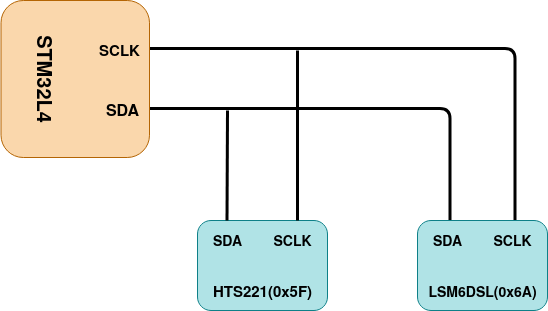
\includegraphics[width=11cm]{source/images/I2C}
	\caption{I2C Kommunikation\label{fig:I2C}}
\end{figure}

\vspace{10cm}
Im Kapitel \ref{Temp} wurde die Funktionsweise beider Sensoren und die 
Vorgehensweise zur Ermittlung der gemessenen Daten behandelt. In diesem 
Abschnitt wird gezeigt wie man Werte im Sensoren-Register schreibt und
wie diese Register zu lesen sind. Im Anhang befinden sich alle Quellen- 
und Header-Dateien. In den Header-Dateien \textbf{hts221.h} und 
\textbf{lsm6dsl.h} sind alle Register (Als Makro-Definition), 
Funktionen zur Initialisierung und zum Auslesen der jeweiligen Sensoren 
definiert. In den Quellen-Dateien \textbf{hts221.c} und 
\textbf{lsm6dsl.c} sind diese Funktionen implementiert. Das folgende 
Textblock zeigt, wie Register gelesen werden und wie man in diesen 
Registern schreiben kann. (Dieses Beispiel bezieht sich auf dem 
HTS221-Sensor)

\begin{lstlisting}[frame=single]
	uint8_t cmd[2];
	cmd[0] = CTRL_REG1;
	i2c_transfer7(I2C2, HTS221_ADDR, cmd, 1, (cmd+1), 1);
	cmd[1] |= (HTS221_PD_ON | HTS221_BDU_ON | HTS221_ODR1_ON);
	i2c_transfer7(I2C2, HTS221_ADDR, cmd, 2, NULL, 0);

\end{lstlisting}
Die Funktion \textbf{i2c\_transfer()} hat sechs Parameter:

\begin{enumerate}
	\item \textbf{i2c:} Die Peripherie, die benutzt wird (Hier I2C2) 
	\item \textbf{addr:} Die Slave-Adresse  
	\item \textbf{w:} Buffer der zu schreibenden Daten
	\item \textbf{wn:} Gr"o\ss{}e der zu schreibenden Daten (In Byte)
	\item \textbf{r:} Buffer, in dem die gelesennen Daten geschrieben 
	werden sollen
	\item \textbf{rn:} Gr"o\ss{}e der zu lesenden Daten (In Byte)
\end{enumerate}

\textbf{Achtung:} Wenn Daten geschrieben werden sollen, ist \textbf{r} 
gleich dem NULL-Pointer und \textbf{rn} gleich null (0), da wir nichts 
lesen wollen.

Diese Vorgehensweise wird (Mit unterschiedlichen Registern) mehrmals 
wiederholt, weil viele Kalibrierregister gelesen und zusammengerechnet 
werden m"ussen, um die gemessenen Werten zu bekommen. Die folgenden 
Textbl"ocke bezeichnen jeweils, wie die Temperatur vom \textbf{HTS221} 
und die Beschleunigung vom \textbf{LSM6DSL} ermittelt werden.

\begin{lstlisting}[frame=single]
	/* Temperatur ermitteln wie im Kapitel 2.1.1 beschrieben */

	/* Read T0_degc_x8 and T1_degc_x8 */
	cmd[0] = TO_DEGC_X8;
	i2c_transfer7(I2C2, HTS221_ADDR, cmd, 1, (cmd+1), 1);
	cmd[0] = T1_DEGC_X8;
	i2c_transfer7(I2C2, HTS221_ADDR, cmd, 1, (cmd+2), 1);

	/* Read the most significant bit of T1_DEGC and T0_DEGC */
	cmd[0] = T1_T0_MSB;
	i2c_transfer7(I2C2, HTS221_ADDR, cmd, 1, (cmd+3), 1);

	/* Calculate the T0_degc and T1_degc values */
	T0_degc_x8 = (((uint16_t)(cmd[3] & 0x02)) << 8) | ((uint16_t)cmd[1]);
	T1_degc_x8 = (((uint16_t)(cmd[3] & 0x0C)) << 6) | ((uint16_t)cmd[2]);
	T0_degc = T0_degc_x8>>3;
	T1_degc = T1_degc_x8>>3;

	/* Read T0_OUT less significant bit */
	cmd[0] = T0_OUT_L;
	i2c_transfer7(I2C2, HTS221_ADDR, cmd, 1, (cmd+1), 1);

	/* Read T0_OUT most significant bit */
	cmd[0] = T0_OUT_M;
	i2c_transfer7(I2C2, HTS221_ADDR, cmd, 1, (cmd+2), 1);
	T0_out = (((int16_t)cmd[2])<<8) | (int16_t)cmd[1];


	/* Read T1_OUT less significant bit */
	cmd[0] = T1_OUT_L;
	i2c_transfer7(I2C2, HTS221_ADDR, cmd, 1, (cmd+1), 1);

	/* Read T1_OUT most significant bit */
	cmd[0] = T1_OUT_M;
	i2c_transfer7(I2C2, HTS221_ADDR, cmd, 1, (cmd+2), 1);
	T1_out = (((int16_t)cmd[2])<<8) | (int16_t)cmd[1];


	/* Read T_OUT less significant bit */
	cmd[0] = T_OUT_L;
	i2c_transfer7(I2C2, HTS221_ADDR, cmd, 1, (cmd+1), 1);

	/* Read T_OUT most significant bit */
	cmd[0] = T_OUT_M;
	i2c_transfer7(I2C2, HTS221_ADDR, cmd, 1, (cmd+2), 1);
	T_out = (((int16_t)cmd[2])<<8) | (int16_t)cmd[1];

	/* Calculate the temperature value */
	tmp = ((int32_t)(T_out - T0_out)) * ((int32_t)(T1_degc - T0_degc));
	temperature = ((float)tmp / (float)(T1_out - T0_out)) + (float)(T0_degc);

	return temperature;
\end{lstlisting}  


\begin{lstlisting}[frame=single]
	/* Beschleunigung ermitteln wie im Abbildung 2.5 */
	
	status_cmd[0] = STATUS_REG;
	i2c_transfer7(I2C2, LSM6DSL_ADDR, status_cmd, 1, (status_cmd+1), 1);
	
	if (status_cmd[1] & GET_XLDA) {
		/* Read X */
		cmd[0] = OUTX_L_XL;
		i2c_transfer7(I2C2, LSM6DSL_ADDR, cmd, 1, (cmd+1), 1);
		outx_l_xl = cmd[1];
	
		cmd[0] = OUTX_H_XL;
		i2c_transfer7(I2C2, LSM6DSL_ADDR, cmd, 1, (cmd+1), 1);
		outx_h_xl = cmd[1];
	
		x = ((int16_t)outx_h_xl << 8 | (int16_t)outx_l_xl);
	
		/* Read Y */
	
		cmd[0] = OUTY_L_XL;
		i2c_transfer7(I2C2, LSM6DSL_ADDR, cmd, 1, (cmd+1), 1);
		outy_l_xl = cmd[1];
	
		cmd[0] = OUTY_H_XL;
		i2c_transfer7(I2C2, LSM6DSL_ADDR, cmd, 1, (cmd+1), 1);
		outy_h_xl = cmd[1];
	
		y = ((int16_t)outy_h_xl << 8 | (int16_t)outy_l_xl);
	
		/* Read Z */
		cmd[0] = OUTZ_L_XL;
		i2c_transfer7(I2C2, LSM6DSL_ADDR, cmd, 1, (cmd+1), 1);
		outz_l_xl = cmd[1];
	
		cmd[0] = OUTZ_H_XL;
		i2c_transfer7(I2C2, LSM6DSL_ADDR, cmd, 1, (cmd+1), 1);
		outz_h_xl = cmd[1];
	
		z = ((int16_t)outz_h_xl << 8 | (int16_t)outz_l_xl);
	
		acc_xyz[0] = (float)x * FS_XL_4G;
		acc_xyz[1] = (float)y * FS_XL_4G;
		acc_xyz[2] = (float)z * FS_XL_4G;
	}
	return acc_xyz;
\end{lstlisting}

\textbf{Achtung:} Die Adresse, die beim Auslesen der Beschleunigung
zur"uckgegeben wird, enth"alt 3 unterschiedliche Werten. Der Index 0 
beinhaltet den Wert der X-Achse, Index 1 beinhaltet den Y-Wert und 
Index 2 den Y-Wert. (Genau so wie f"ur den Gyroskop)

Nachdem die Daten gelesen worden sind, kann man sie nun in Hexadezimal 
konvertieren und mithilfe eines AT-Befehls am Server per LoRaWAN 
senden. Der folgende Abschnitt zeigt, wie das geht.


\section{AT-Kommandos senden}
In diesem Teil geht es haupts"achlich um UART. Die Peripherie muss 
aktiviert und konfiguriert werden, bevor einem Transfer startet. Der 
folgende Quelle-Code ist daf"ur zust"andig.
Die Konfugiration muss die gleiche sein wie im Abschnitt \ref{AT} 
beschrieben (Baudrate: 115200, Daten:8 Bit, keine Parit"at und 1 
Stopbit).

\vspace{1cm}
\begin{lstlisting}[frame=single]
	rcc_periph_clock_enable(RCC_UART4);
	
	void uart_setup(void)
	{
		/* Setup GPIO pins for UART4 and USART3 transmit. */
		gpio_mode_setup(GPIOA, GPIO_MODE_AF, GPIO_PUPD_NONE, GPIO0);
		gpio_mode_setup(GPIOA, GPIO_MODE_AF, GPIO_PUPD_NONE, GPIO1);
	
		/* Setup UART4 TX and RX pin as alternate function. */
		gpio_set_af(GPIOA, GPIO_AF8, GPIO0);
		gpio_set_af(GPIOA, GPIO_AF8, GPIO1);
	
		/* UART4 setup */
		usart_set_baudrate(UART4, 115200);
		usart_set_databits(UART4, 8);
		usart_set_stopbits(UART4, USART_STOPBITS_1);
		usart_set_mode(UART4, USART_MODE_TX_RX);
		usart_set_parity(UART4, USART_PARITY_NONE);
		usart_set_flow_control(UART4, USART_FLOWCONTROL_NONE);
	
		/* Finally enable UART4. */
		usart_enable(UART4);
	}
	
\end{lstlisting}  

Wie im Abschnitt \ref{AT} erw"ahnt, sollen AT-Befehle am LoRa-Modul  
senden, um das Modul f"ur eine LoRaWAN-Verbindung vorzubereiten. Diese 
Befehle werden  ein Zeichen nach dem anderen per UART an dem LoRa-Modul 
gesendet werden. Da viele AT-Befehle Parameter erwarten, haben wir mithilfe
der Stringifikation Makros definiert, die dem Benutzer 
erm"oglichen ver"anderliche Strings in C durch UART zu senden. 

Zuerst wurde eine Enumeration aller Befehle herstellt, die gebraucht 
werden. Danach mithilfe eines zweidimensionalen Feldes und des 
Stingifikation k"onnen wird Parametern zwischen den Strings setzen. Die 
Enumeration gibt den Anfangsindex jedes Befehls an. Damit kann man 
weiter iterieren, um ein kompletes String zu bilden. Die folgenden 
Zeilen-Code zeigen die Stingification, die Enumeration und das 
zweidimensionale Feld.

\vspace{3cm}
\begin{lstlisting}[frame=single]

	/*
	* Stringification
	* Helful to convert macro argument into
	* string constant
	*/
	#define AT_COMMAND(cmd,	param) "AT+" #cmd "=" #param "\r\n\0"
	
\end{lstlisting}     

\begin{lstlisting}[frame=single]
	/*
	* List of possible AT command
	*/
	enum lora_cmd {
		AT = 0,
		ATZ,
		GET_APPEUI,
		GET_EUI,
		GET_NET_S_KEY,
		GET_APP_S_KEY,
		GET_APP_KEY,
		GET_ADDR,
		GET_JOIN_STATUS,
		AT_RADIO,
		AT_GETDATA,
		AT_RX1_DELAY,
		AT_RX2_DELAY,
		AT_JOIN_ACCEPT1_DELAY,
		AT_JOIN_ACCEPT2_DELAY,
		AT_DUTY_CYCLE,
		AT_BAND,
		AT_DATA_RATE,
		AT_RX2_DATA_RATE,
		AT_CLASS,
		AT_ADDR,
		AT_NET_S_KEY,
		AT_APP_S_KEY,
		AT_APP_KEY,
		AT_APPEUI,
		AT_JOIN_OTAA,
		AT_JOIN_ABP,
		AT_NETWORK_TYP,
		AT_ADAPTIVE_DATA_RATE,
		AT_MAX
	};
\end{lstlisting}

\begin{lstlisting}[frame=single]
	/*
	* List of possible codes
	*/
	/* Default network type is public (NTYP = 1, 0 for private network)
	* Band = EU868
	* DevEUI = e24f43fffe44c432
	* Duty Cycle (DC) = is on
	* Data Rate (DR) = SF7/125KHz
	* Class = Class A
	* APPEUI is a 8 bytes hex value
	* AppKey (AK) NSK ASP are 16 byte hex value
	* Device address (ADDR) is a 4 bytes hex value
	* Radio setting: Power: 14dBm
	* 				  Frequency: 867.1MHz
	* 				  Spreading factor: 12
	* 				  Bandwidth: 125KHz
	* 				  Coding rate: 4/5
	*
	*/
	
	char *code[] = {
		"AT\r\n\0",
		"ATZ\r\n\0",
		"AT+APPEUI\r\n\0",
		"AT+EUI\r\n\0",
		"AT+NSK\r\n\0",
		"AT+ASK\r\n\0",
		"AT+AK\r\n\0",
		"AT+ADDR\r\n\0",
		"AT+JSTA\r\n\0",
		"AT+RF=14,8671000000,12,0,1\r\n\0",
		"AT+RCV\r\n\0",
		AT_COMMAND(RX1DT, 1000),
		AT_COMMAND(RX2DT, 2000),
		AT_COMMAND(JRX1DT, 5000),
		AT_COMMAND(JRX2DT, 6000),
		AT_COMMAND(DC, 0),
		AT_COMMAND(BAND, 0),
		AT_COMMAND(DR, 0), //UE860: SF12-BW125
		AT_COMMAND(RX2DR, 0),//UE860: SF12-BW125
		AT_COMMAND(CLASS, 0),
		AT_COMMAND(ADDR, 12345678),
		AT_COMMAND(NSK, 1122334455663EAB546829CB361CAB7D),
		AT_COMMAND(ASK, 887766554433BCFACDE52476CA4598BA),
		AT_COMMAND(AK, 00112233445566778899AABBCCDDEEFF),
		AT_COMMAND(APPEUI, ABC123ADF135CBD8),
		AT_COMMAND(JOIN, 1),
		AT_COMMAND(JOIN, 0),
		AT_COMMAND(NTYP, 1),
		AT_COMMAND(ADR, 1)
	};
\end{lstlisting}

Nun ein Beispiel wie das ganze zu verwenden ist. Jedes Zeichen wird einem nach dem anderen per UART4 gesendet.

\begin{lstlisting}[frame=single]
	void send_cmd(enum lora_cmd cmd)
	{
		char *command = code[cmd];
		/*Send command*/
		if(cmd >= AT_MAX)
			return;
		printf("cmd: %s\n",code[cmd]);
		while (*command != '\0') {
			usart_send_blocking(UART4, *command);
			command++;
		}
	}
\end{lstlisting}

Nachdem ein Befehl gesendet wurde, bekommt man eine Antwort von dem LoRa-Modul zur"uck. 
Diese Antwort ist abh"angig von dem Befehl. Geht es um einen Set-Befehl, bekommt man 
\textbf{OK} oder ein Fehler zur"uck. Ist der Befehle ein Get-Befehl dagegen, bekommt man 
die abgefragte Daten oder ein Fehler zur"uck. Eine Ausnahme besteht bei Events.

Nehmen wir an ein Endger"at m"ochte ein LoRaWAM-Netzwerk eintreten. Das 
Endger"at wird zugelassen, der Server sendet es ein Join-Accept. Diese 
Antwort taucht wie ein Event genau so wie ein normales Downlink auf. 
Diese Antworten werden dann zur P"ufung verwendet oder zur Verarbeitung 
von Downlinks verwendet. Um dieses Verhalten zu visualisieren, wurde 
ein Logic-Analyser namens Saleae \cite{analyzer} verwendet. Das 
folgende Bild zeigt das Ergebnis einer Messung. Es wird ein einfaches 
\textbf{AT} gesendet und das LoRa-Modul antwortet mit \textbf{OK}.

\begin{figure}[h]
	\centering
	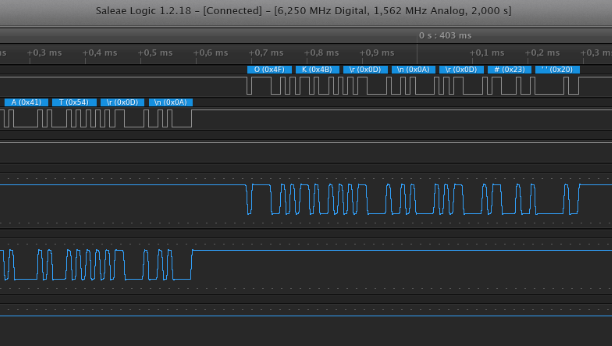
\includegraphics[width=16cm]{source/images/saleae}
	\caption{Verbindungstest mit Saleae\label{fig:saleae}}
\end{figure}

\vspace{5cm}
Diese Antwort wird mithilfe eines Interrupts abgefangen und in einem 
Buffer gespeichert. Um zu pr"ufen, dass ein Befehle richtig interpretiert wurde, wird 
der Inhalt des Antwort-Buffers mit dem String \textbf{OK} mit hilfe der System-Funktion 
\textbf{strcmp()} verglieschen. So k"onnen wir auch pr"ufen ob ein Endger"at dem 
Netzwerk eingetreten ist, indem der Antwort-Buffer mit dem Inhalt des 
Join-Status-Registers. Der Inhalt des Join-Status-Registers ist 1, wenn das Endger"at 
zugelassen wurde, un 0 wenn nicht. So k"onnen wir Join-Request solange senden, bis das 
Endger"at dem Netzwerk zugelassen wird.


\section{Downlinks Behandlung} 

Muss noch Hinzugef"ugt werden.

%Das Fazit
\chapter{Zusammenfassung}\label{Fazit}

F"ur das Ziel dieser Thesis war ich daf"ur 
verantwortlich, ein IoT-Endger"at basierend auf der 
LoRa-Technologie mit einem STM32-Mikrocontroller zu 
entwickeln. Diese IoT-Endger"at erfasst und sammelt 
sowohl Umwelt-Daten, wie Temperatur und Feuchtigkeit, 
als auch die Beschleunigung. Diese Daten werden "uber 
das LoRaWAN-Protokoll an einem Embedded-Linux basiertes 
Gateway gesendet, entweder lokal in diesem Gateway 
verarbeitet oder diesmal "uber das Internet an einem 
Anwendungsserver weitergeleitet. 

Das IoT-Endger"at kann abh"angig des Zwecks 
verschiedene Daten erfassen. Das STM32L4-discovery Kit 
wurde ausgew"ahlt weil es "uber einen eingebetteten 
Debugger/Programmierer, eingebettete Sensoren verf"ugt, 
und leicht erweiterbar ist. Es gibt zwar viele 
LoRa-Module aber allen passen nicht zu der zu 
realisierenden Anwendung. Das i-nucleo-lrwan1 war 
daf"ur geeignet, weil es sich durch UART ansteuern 
l"asst.

\section{Ausblick}

Es k"onnen weitere Endger"ate an dem Netzwerk 
hinzugef"ugt werden. Diese soll einfach nur wie das 
Labcsmart LoRa-endger"at \ref{fig:loranode} 
konfiguriert werden. Die Sensoren k"onnen angepasst 
werden, f"ur die Messung des Stromverbrauchs zum 
Beispiel. Es gibt auch m"oglichkeiten die gemessene 
Daten graphisch darzustellen. 

Dazu muss der MQTT-Broker mit einem Dashboard 
(Open-source, um die Kosten klein wie m"oglich zu 
halten) wie \textbf{Thinkboard} verbunden und 
eingestellt werden. Solche Anwendungen sind 
User-Freundlicher als eine \ac{CSV}-Datei oder die 
Frames, sie in einem Server zu beobachten sind.

\section{Fazit}

Diese Bachelorarbeit war eine gro\ss{}e 
Herausforderung, vor allem wegen der Entscheidung diese 
im Ausland zu absolvieren. Ich konnte viele neue 
Technologien Kennenlernen und diese Praktisch einsetzen. 
Diese Auslandserfahrung  hat mir trotz 
COVID-19-Pendemie sehr gut gefallen. Ich die 
M"oglichkeit Aufgaben selbst"andig zu "ubernehmen, um 
mich praktisch tiefergehend mit den T"atigkeiten 
vertraut zu machen.

Ich habe meine Zeit in Frankreich sehr genossen, da mir 
die Aufgaben sehr gut gefallen haben. Das entspannte 
Arbeitsklima zwischen meinem Chef und mir hatte darauf 
einen gr\ss{}en Einfluss, weil er bei Fragen oder 
Probleme immer verf"ugbar war. Seine Kritiken waren 
auch sehr konstruktiv.  Ich bereue meine Entscheidung, 
im Ausland zu gehen, auf keinen Fall.    

%Einbinden des Abbildungsverzeichnisses


% Quellenverzeichnis
\bibliographystyle{plain}
\bibliography{source/bib/references}

% Anhang
\appendix
\end{document}



%
% EOF
%